\section{Casi d'uso\textsuperscript{G}}
% TEMPLATE
%   \subsection{UC - NomeUseCase}
%   \label{sec:UC}
%   \includegraphics[]{diagramma_UML}
%   \begin{itemize}
	%       \item \textbf{Descrizione:} 
	%       \item \textbf{Attori:} 
	%       \item \textbf{Precondizioni:} 
	%       \item \textbf{Postcondizioni:} 
	%       \item \textbf{Scenario principale:} 
	%       \item \textbf{Generalizzazioni:} 
	%       \item \textbf{Estensioni:} 
	%   \end{itemize}

%   \hyperref[sec:UC]{\textbf{UC}}

% Link ad altre sezioni usando hyperref - utile per linkare generalizzazioni e estensioni
% La label fa da segnalibro a dove dovrà andare il link
%   \label{sec:nomeSezione}
% Link sul quale cliccare per andare alla label
%   \hyperref[sec:nomeSezione]{testo}
% END TEMPLATE

\subsection{Obiettivi}
La sezione ha come obiettivo quello di identificare e descrivere tutti i casi d'uso\textsuperscript{G} che sono stati individuati dal gruppo in sede di analisi del capitolato\textsuperscript{G} assegnato.

\subsection{Attori\textsuperscript{G}}
\begin{wrapfigure}{r}{3.5cm}
	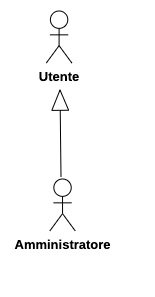
\includegraphics[width=3.5cm]{UML_Use_Cases/UC-Attori.png}
\end{wrapfigure}
Il sistema dispone di due attori principali. In particolare:
\begin{itemize}
	\item \textbf{Utente\textsuperscript{G}}, che accede al servizio come utente\textsuperscript{G} in grado di selezionare una struttura \textit{database\textsuperscript{G}} precaricata, inserire una frase di interrogazione in linguaggio naturale\textsuperscript{G}, visualizzare il \textit{prompt\textsuperscript{G}} generato dall'\textit{LLM\textsuperscript{G}} per poi confermarlo e ottenere una frase in formato \textit{SQL\textsuperscript{G}} che rappresenti quello che era stato richiesto inizialmente.

	\item L'utente\textsuperscript{G} è una generalizzazione dell'amministratore\textsuperscript{G}, il quale accede al servizio con tale ruolo. Oltre a poter compiere tutte le azioni che può fare l'utente\textsuperscript{G} generico, l'amministratore\textsuperscript{G} può creare, visualizzare, modificare ed eliminare un \textit{database\textsuperscript{G}}, le sue tabelle e i suoi campi.
\end{itemize}
% \includegraphics[scale=0.6]{UML_Use_Cases/UC-Attori\textsuperscript{G}.png}

\setcounter{secnumdepth}{0}

\subsection{UC1 - \textit{Login\textsuperscript{G}}}
\label{sec:UC1}
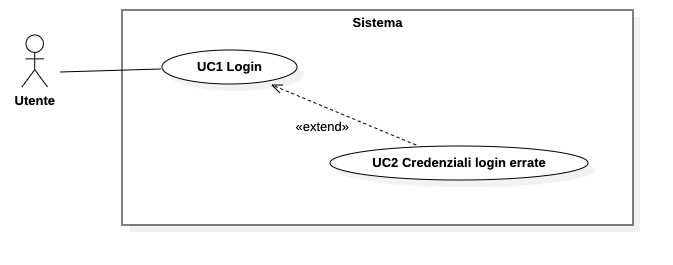
\includegraphics[scale=0.6]{UML_Use_Cases/UC1_2.png}
\begin{itemize}
	\item \textbf{Descrizione:} L’utente\textsuperscript{G} accede al pannello amministrativo con le sue credenziali;
	\item \textbf{Attori\textsuperscript{G}:} Utente\textsuperscript{G};
	\item \textbf{Precondizioni:} 
	\begin{itemize}
		\item L’utente\textsuperscript{G} possiede delle credenziali di accesso valide;
		\item L’utente\textsuperscript{G} non ha già effettuato l’accesso;
	\end{itemize}
	\item \textbf{Postcondizioni:} 
	\begin{itemize}
		\item L’utente\textsuperscript{G} viene riconosciuto dal sistema come amministratore\textsuperscript{G};
	\end{itemize}
	\item \textbf{Scenario principale:} 
	\begin{itemize}
		\item L’ utente\textsuperscript{G} inserisce il proprio nome utente nel \textit{form\textsuperscript{G}} di accesso (\hyperref[sec:UC1.1]{\textbf{UC1.1}});
		\item L’ utente\textsuperscript{G} inserisce la propria \textit{password\textsuperscript{G}} nel \textit{form\textsuperscript{G}} di accesso (\hyperref[sec:UC1.2]{\textbf{UC1.2}});
		\item Il sistema verifica che le credenziali ricevute siano corrette. 
	\end{itemize}
	\item \textbf{Estensioni:} Nel caso le credenziali non siano corrette:
	\begin{itemize}
		\item viene mostrato un errore - \hyperref[sec:UC2]{\textbf{UC2}}
	\end{itemize}
\end{itemize}

\subsubsection{UC1.1 - Inserimento nome utente}
\label{sec:UC1.1}
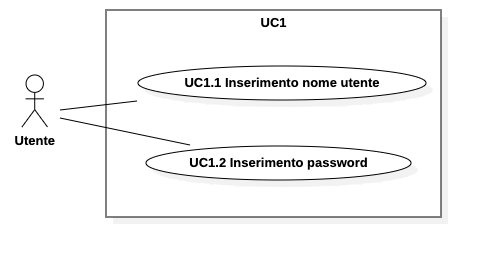
\includegraphics[scale=0.6]{UML_Use_Cases/UC1.1_1.2.png}
\begin{itemize}
	\item \textbf{Descrizione:} L’utente\textsuperscript{G} inserisce il proprio nome utente;
	\item \textbf{Attori\textsuperscript{G}:} utente\textsuperscript{G};
	\item \textbf{Precondizioni:} 
	\begin{itemize}
		\item L’utente\textsuperscript{G} possiede le credenziali di accesso;
		\item L’utente\textsuperscript{G} non ha già effettuato l’accesso;
		\item L’utente\textsuperscript{G} sta effettuando il \textit{login\textsuperscript{G}} (\hyperref[sec:UC1]{\textbf{UC1}})
	\end{itemize}
	\item \textbf{Postcondizioni:} 
	\begin{itemize}
		\item L’utente\textsuperscript{G} ha inserito correttamente il proprio nome utente;
	\end{itemize}
	\item \textbf{Scenario principale:} 
	\begin{itemize}
		\item L’utente\textsuperscript{G} inserisce il proprio nome utente nel \textit{form\textsuperscript{G}} di accesso.
	\end{itemize}
\end{itemize}

\subsubsection{UC1.2 - Inserimento \textit{password\textsuperscript{G}}}
\label{sec:UC1.2}
%\includegraphics[]{diagramma_UML}
\begin{itemize}
	\item \textbf{Descrizione:} L’utente\textsuperscript{G} inserisce la propria \textit{password\textsuperscript{G}};
	\item \textbf{Attori\textsuperscript{G}:} utente\textsuperscript{G};
	\item \textbf{Precondizioni:} 
	\begin{itemize}
		\item L’utente\textsuperscript{G} possiede le credenziali di accesso;
		\item L’utente\textsuperscript{G} non ha già effettuato l’accesso;
		\item L’utente\textsuperscript{G} sta effettuando il \textit{login\textsuperscript{G}} (\hyperref[sec:UC1]{\textbf{UC1}})
	\end{itemize}
	\item \textbf{Postcondizioni:} 
	\begin{itemize}
		\item L’utente\textsuperscript{G} ha inserito correttamente la propria \textit{password\textsuperscript{G}};
	\end{itemize}
	\item \textbf{Scenario principale:} 
	\begin{itemize}
		\item L’utente\textsuperscript{G} inserisce la propria \textit{password\textsuperscript{G}} nel \textit{form\textsuperscript{G}} di accesso.
	\end{itemize}
\end{itemize}

\subsection{UC2 - Credenziali\textsuperscript{G} \textit{login\textsuperscript{G}} errate}
\label{sec:UC2}
%\includegraphics[]{diagramma_UML}
\begin{itemize}
	\item \textbf{Descrizione:} L’utente\textsuperscript{G} visualizza un messaggio di errore di autenticazione;
	\item \textbf{Attori\textsuperscript{G}:} utente\textsuperscript{G};
	\item \textbf{Precondizioni:} 
	\begin{itemize}
		\item L’utente\textsuperscript{G} possiede le credenziali di accesso;
		\item L’utente\textsuperscript{G} non ha già effettuato l’accesso;
		\item L’utente\textsuperscript{G} sta effettuando il \textit{login\textsuperscript{G}} (\hyperref[sec:UC1]{\textbf{UC1}});
		\item L’utente\textsuperscript{G} ha inserito il proprio nome utente\textsuperscript{G} (\hyperref[sec:UC1.1]{\textbf{UC1.1}});
		\item L’utente\textsuperscript{G} ha inserito la propria \textit{password\textsuperscript{G}} (\hyperref[sec:UC1.2]{\textbf{UC1.2}});
	\end{itemize}
	\item \textbf{Postcondizioni:}
	\begin{itemize}
		\item L’utente\textsuperscript{G} non viene riconosciuto dal sistema e deve reinserire le proprie credenziali;
		\item L'utente\textsuperscript{G}  visualizza un messaggio di errore;
	\end{itemize}
	\item \textbf{Scenario principale:} 
	\begin{itemize}
		\item Il sistema verifica le credenziali ricevute siano corrette;
		\item Il sistema visualizza un messaggio di errore per le credenziali inserite se non corrette.
	\end{itemize}
\end{itemize}

\subsection{UC3 - Creazione Struttura \textit{Database}}
\label{sec:UC3}
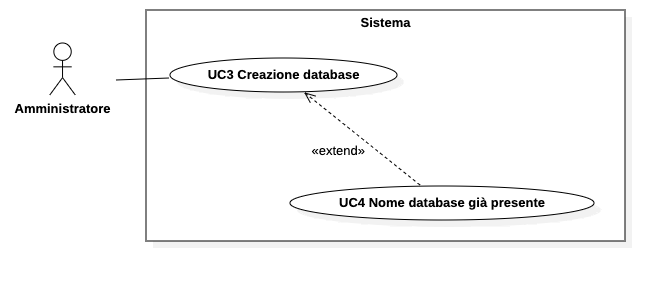
\includegraphics[scale=0.6]{UML_Use_Cases/UC3_4.png}
\begin{itemize}
	\item \textbf{Descrizione:} l’amministratore\textsuperscript{G} vuole aggiungere una struttura  \textit{database\textsuperscript{G}} che l'utente\textsuperscript{G} può interrogare;
	\item \textbf{Attori\textsuperscript{G}:} amministratore\textsuperscript{G};
	\item \textbf{Precondizioni:} 
	\begin{itemize}
		\item L’amministratore\textsuperscript{G} ha effettuato il \textit{login\textsuperscript{G}} (\hyperref[sec:UC1]{\textbf{UC1}});
		\item L’amministratore\textsuperscript{G} si trova nel pannello amministrativo;
	\end{itemize}
	\item \textbf{Postcondizioni:} 
	\begin{itemize}
		\item La struttura \textit{database\textsuperscript{G}} viene salvata nel programma;
	\end{itemize}
	\item \textbf{Scenario principale:} 
	\begin{itemize}
		\item L’amministratore\textsuperscript{G} inserisce il nome (\hyperref[sec:UC3.1]{\textbf{UC3.1}}) e la descrizione (\hyperref[sec:UC3.2]{\textbf{UC3.2}}) della struttura \textit{database\textsuperscript{G}};
	\end{itemize}
	\item \textbf{Estensioni:} nel caso in cui venga inserito un nome già esistente:
	\begin{itemize}
		\item \hyperref[sec:UC4]{\textbf{UC4}} - Errore: nome Struttura \textit{Database}\textsuperscript{G} già presente
	\end{itemize}
\end{itemize}

\subsubsection{UC3.1 - Inserimento nome Struttura \textit{Database}\textsuperscript{G}}
\label{sec:UC3.1}
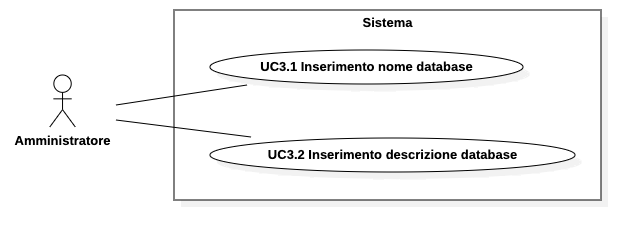
\includegraphics[scale=0.6]{UML_Use_Cases/UC3.1_3.2.png}
\begin{itemize}
	\item \textbf{Descrizione:} l’amministratore\textsuperscript{G} deve inserire il nome della nuova struttura \textit{database\textsuperscript{G}} da aggiungere;
	\item \textbf{Attori\textsuperscript{G}:} amministratore\textsuperscript{G};
	\item \textbf{Precondizioni:} 
	\begin{itemize}
		\item L’amministratore\textsuperscript{G} ha effettuato il \textit{login\textsuperscript{G}} (\hyperref[sec:UC1]{\textbf{UC1}});
		\item L’amministratore\textsuperscript{G} si trova nel pannello amministrativo;
		\item L’amministratore\textsuperscript{G} sta creando un nuovo \textit{database\textsuperscript{G}} (\hyperref[sec:UC3]{\textbf{UC3}});
	\end{itemize}
	\item \textbf{Postcondizioni:} 
	\begin{itemize}
		\item L'amministratore\textsuperscript{G} ha inserito correttamente il nome della nuova struttura  \textit{database\textsuperscript{G}};
	\end{itemize}
	\item \textbf{Scenario principale:} 
	\begin{itemize}
		\item L’amministratore\textsuperscript{G} inserisce il nome della struttura \textit{database\textsuperscript{G}};
	\end{itemize}
\end{itemize}

\subsubsection{UC3.2 - Inserimento descrizione Struttura \textit{Database}\textsuperscript{G}}
\label{sec:UC3.2}
%\includegraphics[]{diagramma_UML}
\begin{itemize}
	\item \textbf{Descrizione:} l’amministratore\textsuperscript{G} deve inserire la descrizione della struttura  \textit{database\textsuperscript{G}} da aggiungere;
	\item \textbf{Attori\textsuperscript{G}:} amministratore\textsuperscript{G};
	\item \textbf{Precondizioni:} 
	\begin{itemize}
		\item L’amministratore\textsuperscript{G} ha effettuato il \textit{login\textsuperscript{G}} (\hyperref[sec:UC1]{\textbf{UC1}});
		\item L’amministratore\textsuperscript{G} si trova nel pannello amministrativo;
		\item L’amministratore\textsuperscript{G} sta creando una nuova struttura \textit{database\textsuperscript{G}} (\hyperref[sec:UC3]{\textbf{UC3}});
	\end{itemize}
	\item \textbf{Postcondizioni:} 
	\begin{itemize}
		\item L'amministratore\textsuperscript{G} ha inserito correttamente la descrizione della struttura  \textit{database\textsuperscript{G}};
	\end{itemize}
	\item \textbf{Scenario principale:} 
	\begin{itemize}
		\item L’amministratore\textsuperscript{G} inserisce la descrizione della Struttura \textit{Database}\textsuperscript{G};
	\end{itemize}
\end{itemize}

\subsection{UC4 - Errore: nome Struttura \textit{Database}\textsuperscript{G} già presente}
\label{sec:UC4}
%\includegraphics[]{diagramma_UML}
\begin{itemize}
	\item \textbf{Descrizione:} L’amministratore\textsuperscript{G} visualizza un errore di creazione della Struttura \textit{Database}\textsuperscript{G};
	\item \textbf{Attori\textsuperscript{G}:} amministratore\textsuperscript{G};
	\item \textbf{Precondizioni:} 
	\begin{itemize}
		\item L’amministratore\textsuperscript{G} ha effettuato il \textit{login\textsuperscript{G}} (\hyperref[sec:UC1]{\textbf{UC1}});
		\item L’amministratore\textsuperscript{G} si trova nel pannello amministrativo;
		\item L’amministratore\textsuperscript{G} sta creando una nuova Struttura \textit{Database\textsuperscript{G}} (\hyperref[sec:UC3]{\textbf{UC3}});
	\end{itemize}
	\item \textbf{Postcondizioni:} 
	\begin{itemize}
		\item La Struttura \textit{Database}\textsuperscript{G} non viene salvata nel programma e l'amministratore\textsuperscript{G} visualizza un messaggio di errore;
	\end{itemize}
	\item \textbf{Scenario principale:} 
	\begin{itemize}
		\item L’amministratore\textsuperscript{G} inserisce il nome della Struttura \textit{Database}\textsuperscript{G} (\hyperref[sec:UC3.1]{\textbf{UC3.1}});
		\item L’amministratore\textsuperscript{G} inserisce la descrizione della Struttura \textit{Database}\textsuperscript{G}  (\hyperref[sec:UC3.2]{\textbf{UC3.2}});
		\item Il sistema verifica che non esista già una struttura \textit{database\textsuperscript{G}} con lo stesso nome;
		\item Il sistema visualizza un messaggio di errore per il nome inserito.
	\end{itemize}
\end{itemize}

\subsection{UC5 - Visualizzazione lista Strutture \textit{Database}\textsuperscript{G}}
\label{sec:UC5}
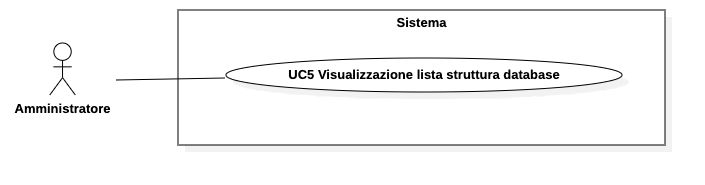
\includegraphics[scale=0.6]{UML_Use_Cases/UC5.png}
\begin{itemize}
	\item \textbf{Descrizione:} l’amministratore\textsuperscript{G} visualizza tutte le Strutture \textit{Database}\textsuperscript{G} disponibili;
	\item \textbf{Attori\textsuperscript{G}:} amministratore\textsuperscript{G};
	\item \textbf{Precondizioni:} 
	\begin{itemize}
		\item L’amministratore\textsuperscript{G} ha effettuato il \textit{login\textsuperscript{G}} (\hyperref[sec:UC1]{\textbf{UC1}});
		\item L’amministratore\textsuperscript{G} si trova nel pannello amministrativo;
	\end{itemize}
	\item \textbf{Postcondizioni:} 
	\begin{itemize}
		\item L'amministratore\textsuperscript{G} può vedere nome e descrizione delle strutture \textit{database}\textsuperscript{G} presenti;
	\end{itemize}
	\item \textbf{Scenario principale:} 
	\begin{itemize}
		\item Il programma visualizza la lista delle strutture \textit{database}\textsuperscript{G} presenti, con la possibilità di modificarle, visualizzarle o eliminarle;
	\end{itemize}
\end{itemize}

\subsection{UC6 - Visualizzazione singola Struttura \textit{Database}\textsuperscript{G}}
\label{sec:UC6}
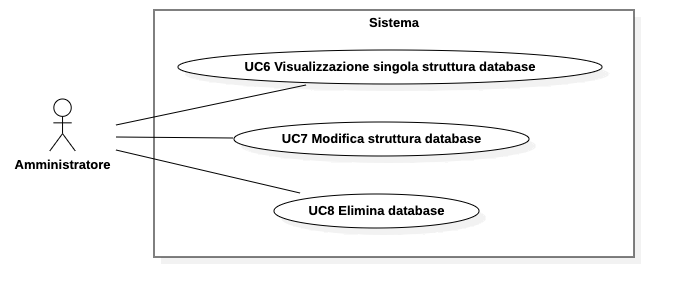
\includegraphics[scale=0.6]{UML_Use_Cases/UC6_7_8.png}
\begin{itemize}
	\item \textbf{Descrizione:} l’amministratore\textsuperscript{G} visualizza una Struttura \textit{Database}\textsuperscript{G};
	\item \textbf{Attori\textsuperscript{G}:} amministratore\textsuperscript{G};
	\item \textbf{Precondizioni:} 
	\begin{itemize}
		\item L’amministratore\textsuperscript{G} ha effettuato il \textit{login\textsuperscript{G}} (\hyperref[sec:UC1]{\textbf{UC1}});
		\item L’amministratore\textsuperscript{G} si trova nel pannello amministrativo;
		\item L'amministratore\textsuperscript{G} ha selezionato una Struttura \textit{Database}\textsuperscript{G} dalla lista;
	\end{itemize}
	\item \textbf{Postcondizioni:} 
	\begin{itemize}
		\item L'amministratore\textsuperscript{G} visualizza il nome della Struttura \textit{Database}\textsuperscript{G};
		\item L'amministratore\textsuperscript{G} visualizza la descrizione della Struttura \textit{Database}\textsuperscript{G};
		\item L'amministratore\textsuperscript{G} visualizza la lista delle tabelle della Struttura \textit{Database}\textsuperscript{G}  (\hyperref[sec:UC11]{\textbf{UC11}};
	\end{itemize}
	\item \textbf{Scenario principale:} 
	\begin{itemize}
		\item Il programma mostra la lista delle Struttura \textit{Database}\textsuperscript{G} presenti, con la possibilità di modificarli, visualizzarli o eliminarli;
	\end{itemize}
\end{itemize}


\subsection{UC7 - Modifica Struttura \textit{Database}\textsuperscript{G}}
\label{sec:UC7}
%\includegraphics[]{diagramma_UML}
\begin{itemize}
	\item \textbf{Descrizione:} l’amministratore\textsuperscript{G} modifica la Struttura \textit{Database}\textsuperscript{G} selezionata;
	\item \textbf{Attori\textsuperscript{G}:} amministratore\textsuperscript{G};
	\item \textbf{Precondizioni:} 
	\begin{itemize}
		\item L’amministratore\textsuperscript{G} sta visualizzando una struttura \textit{Database}\textsuperscript{G} (\hyperref[sec:UC6]{\textbf{UC6}});
	\end{itemize}
	\item \textbf{Postcondizioni:} 
	\begin{itemize}
		\item Il sistema aggiorna la Struttura \textit{Database}\textsuperscript{G};
	\end{itemize}
	\item \textbf{Scenario principale:} 
	\begin{itemize}
		\item L’amministratore\textsuperscript{G} modifica il nome del \textit{Database};
		\item Il sistema verifica il nome ricevuto;
	\end{itemize}
	\item \textbf{Estensioni:} nel caso in cui il nuovo nome sia già presente:
	\begin{itemize}
		\item \hyperref[sec:UC4]{\textbf{UC4}} - Errore: nome Struttura \textit{Database} già presente.
	\end{itemize}
\end{itemize}

\subsection{UC8 - Elimina Struttura \textit{Database}\textsuperscript{G}}
\label{sec:UC8}
%\includegraphics[]{diagramma_UML}
\begin{itemize}
	\item \textbf{Descrizione:} l’amministratore\textsuperscript{G} elimina la Struttura \textit{Database}\textsuperscript{G} selezionata;
	\item \textbf{Attori\textsuperscript{G}:} amministratore\textsuperscript{G};
	\item \textbf{Precondizioni:} 
	\begin{itemize}
		\item L’amministratore\textsuperscript{G} ha effettuato il \textit{login\textsuperscript{G}} (\hyperref[sec:UC1]{\textbf{UC1}});
		\item L’amministratore\textsuperscript{G} si trova nel pannello amministrativo;
		\item L’amministratore\textsuperscript{G} sta visualizzando la lista delle Strutture \textit{Database}\textsuperscript{G} (\hyperref[sec:UC5]{\textbf{UC5}});
	\end{itemize}
	\item \textbf{Postcondizioni:} 
	\begin{itemize}
		\item La Struttura \textit{Database}\textsuperscript{G} selezionata viene eliminata dal sistema;
	\end{itemize}
	\item \textbf{Scenario principale:} 
	\begin{itemize}
		\item L'amministratore\textsuperscript{G} seleziona la Struttura \textit{database}\textsuperscript{G} da eliminare usando il pulsante di eliminazione apposito;
		\item Il sistema visualizza un messaggio per chiedere la conferma dell'eliminazione;
		\item Se l'amministratore\textsuperscript{G} conferma l'eliminazione, la Struttura \textit{Database}\textsuperscript{G} e le tabelle collegate verranno rimossi dal sistema e verrà visualizzato un messaggio di avvenuta eliminazione.
	\end{itemize}
\end{itemize}

\subsection{UC9 - Creazione tabella\textsuperscript{G} Struttura \textit{Database}\textsuperscript{G}}
\label{sec:UC9}
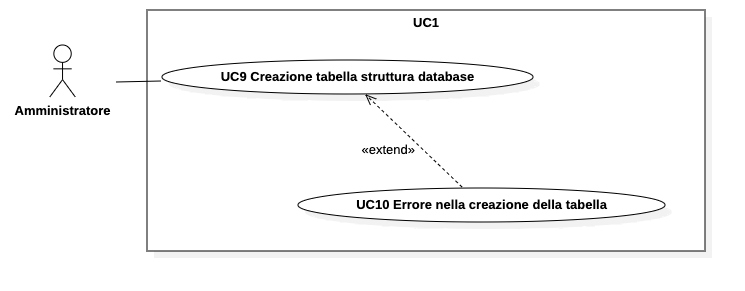
\includegraphics[scale=0.6]{UML_Use_Cases/UC9_10.png}
\begin{itemize}
	\item \textbf{Descrizione:} l’amministratore\textsuperscript{G} vuole aggiungere una tabella\textsuperscript{G} ad una Struttura \textit{Database}\textsuperscript{G};
	\item \textbf{Attori\textsuperscript{G}:} amministratore\textsuperscript{G};
	\item \textbf{Precondizioni:} 
	\begin{itemize}
		\item L’amministratore\textsuperscript{G} ha effettuato il \textit{login\textsuperscript{G}} (\hyperref[sec:UC1]{\textbf{UC1}});
		\item L’amministratore\textsuperscript{G} si trova nel pannello amministrativo;
		\item L’amministratore\textsuperscript{G} si trova nella sezione di creazione di una nuova tabella\textsuperscript{G};
	\end{itemize}
	\item \textbf{Postcondizioni:} 
	\begin{itemize}
		\item La tabella\textsuperscript{G} viene aggiunta alla struttura della Struttura \textit{Database}\textsuperscript{G};
	\end{itemize}
	\item \textbf{Scenario principale:} 
	\begin{itemize}
		\item L’amministratore\textsuperscript{G} inserisce il nome, i sinonimi\textsuperscript{G} del nome e la descrizione della tabella\textsuperscript{G};
	\end{itemize}
	\item \textbf{Generalizzazioni:} 
	\begin{itemize}
		\item \hyperref[sec:UC9.1]{\textbf{UC9.1}} - Inserimento nome tabella\textsuperscript{G}
		\item \hyperref[sec:UC9.2]{\textbf{UC9.2}} - Inserimento sinonimi\textsuperscript{G} tabella\textsuperscript{G}
		\item \hyperref[sec:UC9.3]{\textbf{UC9.3}} - Inserimento descrizione tabella\textsuperscript{G}
	\end{itemize}
	\item \textbf{Estensioni:} nel caso in cui non vengano inseriti i sinonimi\textsuperscript{G} del nome della tabella\textsuperscript{G}, o il nome esisti già:
	\begin{itemize}
		\item \hyperref[sec:UC10]{\textbf{UC10}} - Errore nella creazione della tabella\textsuperscript{G}
	\end{itemize}
\end{itemize}

\subsubsection{UC9.1 - Inserimento nome tabella\textsuperscript{G}}
\label{sec:UC9.1}
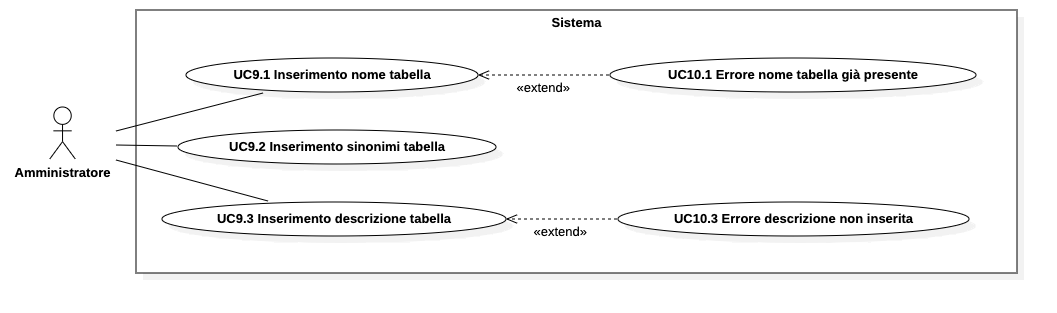
\includegraphics[scale=0.47]{UML_Use_Cases/UC9.1_9.2_9.3_10.1_10.2_10.3.png}
\begin{itemize}
	\item \textbf{Descrizione:} l’amministratore\textsuperscript{G} inserisce il nome della tabella\textsuperscript{G} da creare;
	\item \textbf{Attori\textsuperscript{G}:} amministratore\textsuperscript{G};
	\item \textbf{Precondizioni:} 
	\begin{itemize}
		\item L’amministratore\textsuperscript{G} ha effettuato il \textit{login\textsuperscript{G}} (\hyperref[sec:UC1]{\textbf{UC1}});
		\item L’amministratore\textsuperscript{G} sta creando una nuova tabella\textsuperscript{G} (\hyperref[sec:UC9]{\textbf{UC9}});
	\end{itemize}
	\item \textbf{Postcondizioni:} 
	\begin{itemize}
		\item Il nome della tabella\textsuperscript{G} viene inserito nel \textit{form\textsuperscript{G}};
	\end{itemize}
	\item \textbf{Scenario principale:} 
	\begin{itemize}
		\item L’amministratore\textsuperscript{G} inserisce il nome della tabella\textsuperscript{G} nell'apposito \textit{form\textsuperscript{G}} di creazione;
	\end{itemize}
\end{itemize}

\subsubsection{UC9.2 - Inserimento sinonimi\textsuperscript{G} tabella\textsuperscript{G}}
\label{sec:UC9.2}
%\includegraphics[]{diagramma_UML}
\begin{itemize}
	\item \textbf{Descrizione:} l’amministratore\textsuperscript{G} inserisce i sinonimi\textsuperscript{G} associati al nome della tabella\textsuperscript{G} da creare;
	\item \textbf{Attori\textsuperscript{G}:} amministratore\textsuperscript{G};
	\item \textbf{Precondizioni:} 
	\begin{itemize}
		\item L’amministratore\textsuperscript{G} ha effettuato il \textit{login\textsuperscript{G}} (\hyperref[sec:UC1]{\textbf{UC1}});
		\item L’amministratore\textsuperscript{G} sta creando una nuova tabella\textsuperscript{G} (\hyperref[sec:UC9]{\textbf{UC9}});
	\end{itemize}
	\item \textbf{Postcondizioni:} 
	\begin{itemize}
		\item I sinonimi\textsuperscript{G} della tabella\textsuperscript{G} vengono inseriti nel \textit{form\textsuperscript{G}};
	\end{itemize}
	\item \textbf{Scenario principale:} 
	\begin{itemize}
		\item L’amministratore\textsuperscript{G} inserisce i sinonimi\textsuperscript{G} del nome della tabella\textsuperscript{G} nell'apposito \textit{form\textsuperscript{G}} di creazione;
	\end{itemize}
\end{itemize}

\subsubsection{UC9.3 - Inserimento descrizione tabella\textsuperscript{G}}
\label{sec:UC9.3}
%\includegraphics[]{diagramma_UML}
\begin{itemize}
	\item \textbf{Descrizione:} l’amministratore\textsuperscript{G} inserisce la descrizione della tabella\textsuperscript{G} da creare;
	\item \textbf{Attori\textsuperscript{G}:} amministratore\textsuperscript{G};
	\item \textbf{Precondizioni:} 
	\begin{itemize}
		\item L’amministratore\textsuperscript{G} ha effettuato il \textit{login\textsuperscript{G}} (\hyperref[sec:UC1]{\textbf{UC1}});
		\item L’amministratore\textsuperscript{G} sta creando una nuova tabella\textsuperscript{G} (\hyperref[sec:UC9]{\textbf{UC9}});
	\end{itemize}
	\item \textbf{Postcondizioni:} 
	\begin{itemize}
		\item La descrizione della tabella\textsuperscript{G} viene inserita nel \textit{form\textsuperscript{G}};
	\end{itemize}
	\item \textbf{Scenario principale:} 
	\begin{itemize}
		\item L’amministratore\textsuperscript{G} inserisce la descrizione della tabella\textsuperscript{G} nell'apposito \textit{form\textsuperscript{G}} di creazione;
	\end{itemize}
\end{itemize}

\subsection{UC10 - Errore nella creazione della tabella\textsuperscript{G}}
\label{sec:UC10}
%\includegraphics[]{diagramma_UML}
\begin{itemize}
	\item \textbf{Descrizione:} L’amministratore\textsuperscript{G} visualizza un errore di creazione della tabella\textsuperscript{G};
	\item \textbf{Attori\textsuperscript{G}:} amministratore\textsuperscript{G};
	\item \textbf{Precondizioni:} 
	\begin{itemize}
		\item L’amministratore\textsuperscript{G} ha effettuato il \textit{login\textsuperscript{G}} (\hyperref[sec:UC1]{\textbf{UC1}});
		\item L’amministratore\textsuperscript{G} sta creando una nuova tabella\textsuperscript{G} (\hyperref[sec:UC9]{\textbf{UC9}});
	\end{itemize}
	\item \textbf{Postcondizioni:} 
	\begin{itemize}
		\item La tabella\textsuperscript{G} non viene creata e il programma visualizza un messaggio di errore;
	\end{itemize}
	\item \textbf{Scenario principale:} 
	\begin{itemize}
		\item L’amministratore\textsuperscript{G} inserisce il nome della tabella\textsuperscript{G} nel \textit{form\textsuperscript{G}} di creazione (\hyperref[sec:UC9.1]{\textbf{UC9.1}});
		\item L’amministratore\textsuperscript{G} inserisce i sinonimi\textsuperscript{G} del nome della tabella\textsuperscript{G} nel \textit{form\textsuperscript{G}} di creazione (\hyperref[sec:UC9.2]{\textbf{UC9.2}});
		\item L’amministratore\textsuperscript{G} inserisce la descrizione della tabella\textsuperscript{G} nel \textit{form\textsuperscript{G}} di creazione (\hyperref[sec:UC9.3]{\textbf{UC9.3}});
		\item Il sistema verifica che non esista già una tabella\textsuperscript{G} con lo stesso nome e che vengano inseriti sinonimi\textsuperscript{G} e descrizione della tabella\textsuperscript{G};
		\item Il sistema visualizza il messaggio di errore opportuno.
	\end{itemize}
\end{itemize}

\subsubsection{UC10.1 - Errore nome tabella\textsuperscript{G} già presente}
\label{sec:UC10.1}
%\includegraphics[]{diagramma_UML}
\begin{itemize}
	\item \textbf{Descrizione:} L’amministratore\textsuperscript{G} visualizza un errore relativo al nome della tabella\textsuperscript{G};
	\item \textbf{Attori\textsuperscript{G}:} amministratore\textsuperscript{G};
	\item \textbf{Precondizioni:} 
	\begin{itemize}
		\item L’amministratore\textsuperscript{G} ha effettuato il \textit{login\textsuperscript{G}} (\hyperref[sec:UC1]{\textbf{UC1}});
		\item L’amministratore\textsuperscript{G} sta creando una nuova tabella\textsuperscript{G} (\hyperref[sec:UC9]{\textbf{UC9}});
	\end{itemize}
	\item \textbf{Postcondizioni:} 
	\begin{itemize}
		\item La tabella\textsuperscript{G} non viene creata e il programma visualizza un messaggio di errore;
	\end{itemize}
	\item \textbf{Scenario principale:} 
	\begin{itemize}
		\item Il sistema verifica che non esista già una tabella\textsuperscript{G} con lo stesso nome;
		\item Il sistema visualizza il messaggio di errore per il nome inserito.
	\end{itemize}
\end{itemize}

\subsubsection{UC10.2 - Errore sinonimi\textsuperscript{G} non inseriti}
\label{sec:UC10.2}
%\includegraphics[]{diagramma_UML}
\begin{itemize}
	\item \textbf{Descrizione:} L’amministratore\textsuperscript{G} visualizza un errore relativo ai sinonimi\textsuperscript{G} del nome della tabella\textsuperscript{G};
	\item \textbf{Attori\textsuperscript{G}:} amministratore\textsuperscript{G};
	\item \textbf{Precondizioni:} 
	\begin{itemize}
		\item L’amministratore\textsuperscript{G} ha effettuato il \textit{login\textsuperscript{G}} (\hyperref[sec:UC1]{\textbf{UC1}});
		\item L’amministratore\textsuperscript{G} sta creando una nuova tabella\textsuperscript{G} (\hyperref[sec:UC9]{\textbf{UC9}});
	\end{itemize}
	\item \textbf{Postcondizioni:} 
	\begin{itemize}
		\item La tabella\textsuperscript{G} non viene creata e il programma visualizza un messaggio di errore;
	\end{itemize}
	\item \textbf{Scenario principale:} 
	\begin{itemize}
		\item Il sistema verifica che il campo\textsuperscript{G} relativo ai sinonimi\textsuperscript{G} del nome della tabella\textsuperscript{G} non sia vuoto;
		\item Il sistema visualizza il messaggio di errore per il campo\textsuperscript{G} sinonimi\textsuperscript{G} vuoto.
	\end{itemize}
\end{itemize}

\subsubsection{UC10.3 - Errore descrizione non inserita}
\label{sec:UC10.3}
%\includegraphics[]{diagramma_UML}
\begin{itemize}
	\item \textbf{Descrizione:} L’amministratore\textsuperscript{G} visualizza un errore relativo alla descrizione della tabella\textsuperscript{G};
	\item \textbf{Attori\textsuperscript{G}:} amministratore\textsuperscript{G};
	\item \textbf{Precondizioni:} 
	\begin{itemize}
		\item L’amministratore\textsuperscript{G} ha effettuato il \textit{login\textsuperscript{G}} (\hyperref[sec:UC1]{\textbf{UC1}});
		\item L’amministratore\textsuperscript{G} sta creando una nuova tabella\textsuperscript{G} (\hyperref[sec:UC9]{\textbf{UC9}});
	\end{itemize}
	\item \textbf{Postcondizioni:} 
	\begin{itemize}
		\item La tabella\textsuperscript{G} non viene creata e il programma visualizza un messaggio di errore;
	\end{itemize}
	\item \textbf{Scenario principale:} 
	\begin{itemize}
		\item Il sistema verifica che il campo\textsuperscript{G} relativo ai sinonimi\textsuperscript{G} del nome della tabella\textsuperscript{G} non sia vuoto;
		\item Il sistema visualizza il messaggio di errore per il campo\textsuperscript{G} descrizione vuoto.
	\end{itemize}
\end{itemize}

\subsection{UC11 - Visualizzazione lista delle tabelle nella Struttura \textit{Database}\textsuperscript{G}}
\label{sec:UC11}
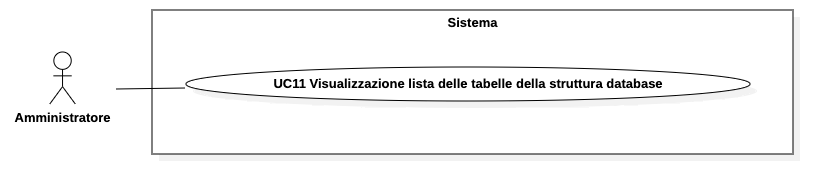
\includegraphics[scale=0.6]{UML_Use_Cases/UC11.png}
\begin{itemize}
	\item \textbf{Descrizione:} l’amministratore\textsuperscript{G} visualizza tutte le tabelle della Struttura \textit{Database}\textsuperscript{G} selezionata;
	\item \textbf{Attori\textsuperscript{G}:} amministratore\textsuperscript{G};
	\item \textbf{Precondizioni:} 
	\begin{itemize}
		\item L’amministratore\textsuperscript{G} ha effettuato il \textit{login\textsuperscript{G}} (\hyperref[sec:UC1]{\textbf{UC1}});
		\item L’amministratore\textsuperscript{G} si trova nel pannello amministrativo;
		\item L'amministratore\textsuperscript{G} ha selezionato una Struttura \textit{Database}\textsuperscript{G} dalla lista;
	\end{itemize}
	\item \textbf{Postcondizioni:} 
	\begin{itemize}
		\item L'amministratore\textsuperscript{G} può vedere il nome delle tabelle presenti;
	\end{itemize}
	\item \textbf{Scenario principale:} 
	\begin{itemize}
		\item Il programma visualizza la lista delle tabelle presenti, con la possibilità di modificarle, visualizzarle o eliminarle;
	\end{itemize}
\end{itemize}

\subsection{UC12 - Visualizzazione della singola tabella\textsuperscript{G}}
\label{sec:UC12}
%\includegraphics[]{diagramma_UML}
\begin{itemize}
	\item \textbf{Descrizione:} l’amministratore\textsuperscript{G} visualizza la tabella\textsuperscript{G} della Struttura \textit{Database}\textsuperscript{G} selezionata;
	\item \textbf{Attori\textsuperscript{G}:} amministratore\textsuperscript{G};
	\item \textbf{Precondizioni:} 
	\begin{itemize}
		\item L'amministratore\textsuperscript{G} ha visualizzato la lista delle tabelle della Struttura \textit{Database}\textsuperscript{G} (\hyperref[sec:UC11]{\textbf{UC11}});
		\item L'amministratore\textsuperscript{G} ha selezionato una tabella\textsuperscript{G} dalla lista;
	\end{itemize}
	\item \textbf{Postcondizioni:} 
	\begin{itemize}
		\item L'amministratore\textsuperscript{G} può vedere nome, descrizione e sinonimi\textsuperscript{G} della tabella\textsuperscript{G} selezionata;
		\item L'amministratore\textsuperscript{G} può visualizzare i campi della tabella\textsuperscript{G} selezionata;
	\end{itemize}
	\item \textbf{Scenario principale:} 
	\begin{itemize}
		\item Il programma visualizza i campi della tabella\textsuperscript{G} selezionata;
	\end{itemize}
\end{itemize}

\subsection{UC13 - Modifica della tabella\textsuperscript{G}}
\label{sec:UC13}
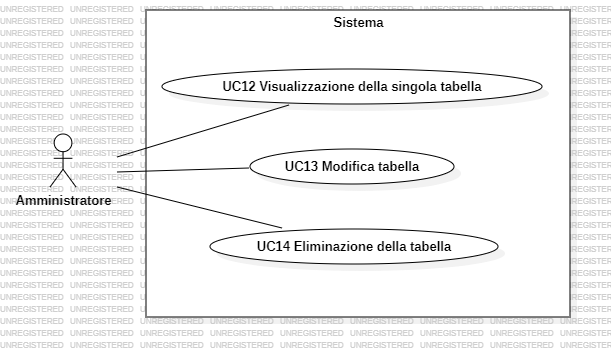
\includegraphics[scale=0.6]{UML_Use_Cases/UC12_13_14.png}
\begin{itemize}
	\item \textbf{Descrizione:} l’amministratore\textsuperscript{G} vuole modificare una tabella\textsuperscript{G} della Struttura \textit{Database}\textsuperscript{G} selezionato e da interrogare;
	\item \textbf{Attori\textsuperscript{G}:} amministratore\textsuperscript{G};
	\item \textbf{Precondizioni:} 
	\begin{itemize}
		\item L’amministratore\textsuperscript{G} ha effettuato il \textit{login\textsuperscript{G}} (\hyperref[sec:UC1]{\textbf{UC1}});
		\item L’amministratore\textsuperscript{G} si trova nel pannello amministrativo;
		\item L’amministratore\textsuperscript{G} si trova nella sezione di modifica di una tabella\textsuperscript{G};
	\end{itemize}
	\item \textbf{Postcondizioni:} 
	\begin{itemize}
		\item La tabella\textsuperscript{G} selezionata viene modificata;
	\end{itemize}
	\item \textbf{Scenario principale:} 
	\begin{itemize}
		\item L’amministratore\textsuperscript{G} modifica il nome, i sinonimi\textsuperscript{G} del nome e la descrizione della tabella\textsuperscript{G};
	\end{itemize}
	\item \textbf{Estensioni:} nel caso in cui non vengano rimossi completamente i sinonimi\textsuperscript{G} del nome della tabella\textsuperscript{G}, o il nome modificato è già presente:
	\begin{itemize}
		\item \hyperref[sec:UC10]{\textbf{UC10}} - Errore nella creazione della tabella\textsuperscript{G}
	\end{itemize}
\end{itemize}

\subsection{UC14 - Eliminazione della tabella\textsuperscript{G}}
\label{sec:UC14}
%\includegraphics[]{diagramma_UML}
\begin{itemize}
	\item \textbf{Descrizione:} l’amministratore\textsuperscript{G} elimina la tabella\textsuperscript{G} selezionata;
	\item \textbf{Attori\textsuperscript{G}:} amministratore\textsuperscript{G};
	\item \textbf{Precondizioni:} 
	\begin{itemize}
		\item L’amministratore\textsuperscript{G} ha effettuato il \textit{login\textsuperscript{G}} (\hyperref[sec:UC1]{\textbf{UC1}});
		\item L’amministratore\textsuperscript{G} si trova nel pannello amministrativo;
		\item L’amministratore\textsuperscript{G} sta visualizzando la lista delle tabelle (\hyperref[sec:UC11]{\textbf{UC11}});
	\end{itemize}
	\item \textbf{Postcondizioni:} 
	\begin{itemize}
		\item La Struttura \textit{Database}\textsuperscript{G} selezionata viene eliminata dal sistema;
	\end{itemize}
	\item \textbf{Scenario principale:} 
	\begin{itemize}
		\item L'amministratore\textsuperscript{G} seleziona la tabella\textsuperscript{G} da eliminare usando il pulsante di eliminazione apposito;
		\item Il sistema visualizza un messaggio per chiedere la conferma dell'eliminazione;
		\item Se l'amministratore\textsuperscript{G} conferma l'eliminazione, la tabella\textsuperscript{G} e i suoi campi verranno rimossi dal sistema e verrà visualizzato un messaggio di avvenuta eliminazione.
	\end{itemize}
\end{itemize}

\subsection{UC15 - Creazione campo\textsuperscript{G} tabella\textsuperscript{G}}
\label{sec:UC15}
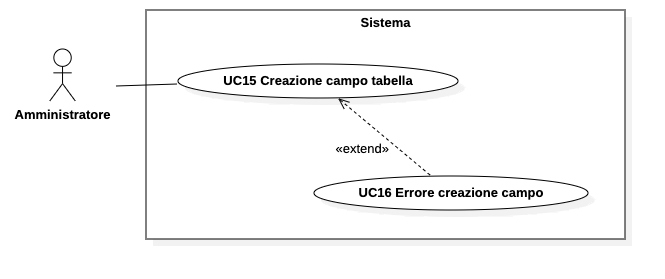
\includegraphics[scale=0.6]{UML_Use_Cases/UC15_16.png}
\begin{itemize}
	\item \textbf{Descrizione:} l’amministratore\textsuperscript{G} vuole aggiungere un campo\textsuperscript{G} alla tabella\textsuperscript{G} selezionata;
	\item \textbf{Attori\textsuperscript{G}:} amministratore\textsuperscript{G};
	\item \textbf{Precondizioni:} 
	\begin{itemize}
		\item L’amministratore\textsuperscript{G} ha effettuato il \textit{login\textsuperscript{G}} (\hyperref[sec:UC1]{\textbf{UC1}});
		\item L’amministratore\textsuperscript{G} si trova nel pannello amministrativo;
		\item L’amministratore\textsuperscript{G} si trova nella sezione di visualizzazione di una tabella\textsuperscript{G} (\hyperref[sec:UC12]{\textbf{UC12}});
		\item L’amministratore\textsuperscript{G} sta inserendo i campi che compongono la tabella\textsuperscript{G};
	\end{itemize}
	\item \textbf{Postcondizioni:} 
	\begin{itemize}
		\item I campi vengono aggiunti alla tabella\textsuperscript{G};
	\end{itemize}
	\item \textbf{Scenario principale:} 
	\begin{itemize}
		\item L’amministratore\textsuperscript{G} inserisce il nome del campo\textsuperscript{G} \hyperref[sec:UC15.1]{\textbf{UC15.1}};
		\item L'amministratore\textsuperscript{G} seleziona il tipo del campo\textsuperscript{G} \hyperref[sec:UC15.2]{\textbf{UC15.2}};
		\item L'amministratore\textsuperscript{G} inserisce i sinonimi\textsuperscript{G} del campo\textsuperscript{G} \hyperref[sec:UC15.3]{\textbf{UC15.3}};
	\end{itemize}
	\item \textbf{Estensioni:} nel caso in cui il nome inserito sia già esistente o non sia stato selezionato il tipo o inseriti i sinonimi\textsuperscript{G}:
	\begin{itemize}
		\item \hyperref[sec:UC16]{\textbf{UC16}} - Errore creazione campo\textsuperscript{G}
	\end{itemize}
\end{itemize}

\subsubsection{UC15.1 - Inserimento nome campo\textsuperscript{G}}
\label{sec:UC15.1}
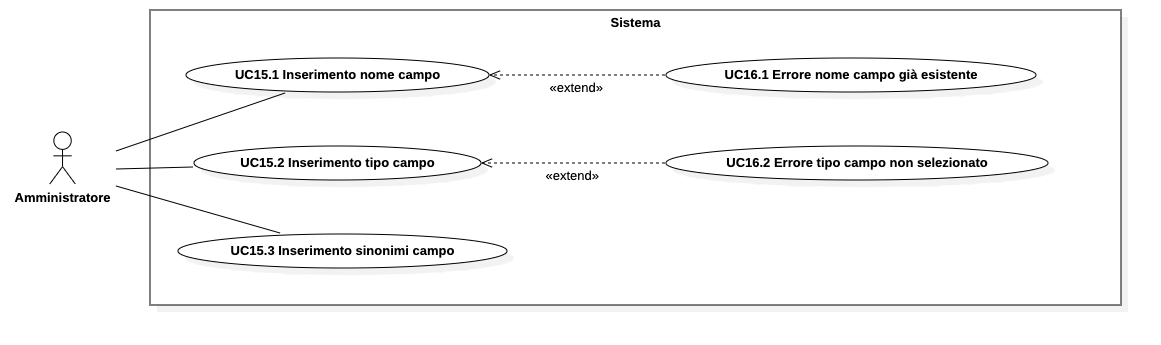
\includegraphics[scale=0.45]{UML_Use_Cases/UC15.1_15.2_15.3_16.1_16.2_16.3.png}
\begin{itemize}
	\item \textbf{Descrizione:} l’amministratore\textsuperscript{G} vuole inserire il nome del campo\textsuperscript{G} da inserire nella tabella\textsuperscript{G};
	\item \textbf{Attori\textsuperscript{G}:} amministratore\textsuperscript{G};
	\item \textbf{Precondizioni:} 
	\begin{itemize}
		\item L’amministratore\textsuperscript{G} ha effettuato il \textit{login\textsuperscript{G}} (\hyperref[sec:UC1]{\textbf{UC1}});
		\item L’amministratore\textsuperscript{G} si trova nel pannello amministrativo;
		\item L’amministratore\textsuperscript{G} si trova nella sezione di visualizzazione di una tabella\textsuperscript{G} (\hyperref[sec:UC12]{\textbf{UC12}});
		\item L’amministratore\textsuperscript{G} sta inserendo i campi che compongono la tabella\textsuperscript{G};
	\end{itemize}
	\item \textbf{Postcondizioni:} 
	\begin{itemize}
		\item Il nome del campo\textsuperscript{G} viene inserito;
	\end{itemize}
	\item \textbf{Scenario principale:} 
	\begin{itemize}
		\item L’amministratore\textsuperscript{G} inserisce il nome del campo\textsuperscript{G} nella casella di testo dedicata;
	\end{itemize}
	\item \textbf{Estensioni:} nel caso in cui il nome inserito sia già esistente:
	\begin{itemize}
		\item \hyperref[sec:UC16.1]{\textbf{UC16.1}} - Errore nome campo\textsuperscript{G} già esistente
	\end{itemize}
\end{itemize}

\subsubsection{UC15.2 - Inserimento tipo campo\textsuperscript{G}}
\label{sec:UC15.2}
%\includegraphics[]{diagramma_UML}
\begin{itemize}
	\item \textbf{Descrizione:} l’amministratore\textsuperscript{G} vuole selezionare il tipo del campo\textsuperscript{G} da inserire nella tabella\textsuperscript{G};
	\item \textbf{Attori\textsuperscript{G}:} amministratore\textsuperscript{G};
	\item \textbf{Precondizioni:} 
	\begin{itemize}
		\item L’amministratore\textsuperscript{G} ha effettuato il \textit{login\textsuperscript{G}} (\hyperref[sec:UC1]{\textbf{UC1}});
		\item L’amministratore\textsuperscript{G} si trova nel pannello amministrativo;
		\item L’amministratore\textsuperscript{G} si trova nella sezione di visualizzazione di una tabella\textsuperscript{G} (\hyperref[sec:UC12]{\textbf{UC12}}) ;
		\item L’amministratore\textsuperscript{G} sta inserendo i campi che compongono la tabella\textsuperscript{G};
	\end{itemize}
	\item \textbf{Postcondizioni:} 
	\begin{itemize}
		\item Il tipo del campo\textsuperscript{G} viene selezionato;
	\end{itemize}
	\item \textbf{Scenario principale:} 
	\begin{itemize}
		\item L’amministratore\textsuperscript{G} sceglie il tipo di campo\textsuperscript{G}, selezionandolo dalle scelte possibili;
	\end{itemize}
	\item \textbf{Estensioni:} nel caso in cui il tipo non venga selezionato:
	\begin{itemize}
		\item \hyperref[sec:UC16.2]{\textbf{UC16.2}} - Errore tipo campo\textsuperscript{G} non selezionato
	\end{itemize}
\end{itemize}

\subsubsection{UC15.3 - Inserimento sinonimi\textsuperscript{G} campo\textsuperscript{G}}
\label{sec:UC15.3}
%\includegraphics[]{diagramma_UML}
\begin{itemize}
	\item \textbf{Descrizione:} l’amministratore\textsuperscript{G} vuole inserire i sinonimi\textsuperscript{G} del campo\textsuperscript{G} da inserire nella tabella\textsuperscript{G};
	\item \textbf{Attori\textsuperscript{G}:} amministratore\textsuperscript{G};
	\item \textbf{Precondizioni:} 
	\begin{itemize}
		\item L’amministratore\textsuperscript{G} ha effettuato il \textit{login\textsuperscript{G}} (\hyperref[sec:UC1]{\textbf{UC1}});
		\item L’amministratore\textsuperscript{G} si trova nel pannello amministrativo;
		\item L’amministratore\textsuperscript{G} si trova nella sezione di visualizzazione di una tabella\textsuperscript{G} (\hyperref[sec:UC12]{\textbf{UC12}} ;
		\item L’amministratore\textsuperscript{G} sta inserendo i campi che compongono la tabella\textsuperscript{G};
	\end{itemize}
	\item \textbf{Postcondizioni:} 
	\begin{itemize}
		\item I sinonimi\textsuperscript{G} del nome del campo\textsuperscript{G} vengono inseriti;
	\end{itemize}
	\item \textbf{Scenario principale:} 
	\begin{itemize}
		\item L’amministratore\textsuperscript{G} inserisce i sinonimi\textsuperscript{G} del nome del campo\textsuperscript{G} nella casella di testo dedicata;
	\end{itemize}
	\item \textbf{Estensioni:} nel caso in cui i sinonimi\textsuperscript{G} non vengano inseriti:
	\begin{itemize}
		\item \hyperref[sec:UC16.3]{\textbf{UC16.3}} - Errore mancato inserimento sinonimi\textsuperscript{G} campo\textsuperscript{G}
	\end{itemize}
\end{itemize}

\subsection{UC16 - Errore creazione campo\textsuperscript{G}}
\label{sec:UC16}
%\includegraphics[]{diagramma_UML}
\begin{itemize}
	\item \textbf{Descrizione:} L’amministratore\textsuperscript{G} visualizza un errore di creazione del campo\textsuperscript{G};
	\item \textbf{Attori\textsuperscript{G}:} amministratore\textsuperscript{G};
	\item \textbf{Precondizioni:} 
	\begin{itemize}
		\item L’amministratore\textsuperscript{G} ha effettuato il \textit{login\textsuperscript{G}} (\hyperref[sec:UC1]{\textbf{UC1}});
		\item L’amministratore\textsuperscript{G} si trova nel pannello amministrativo;
		\item L’amministratore\textsuperscript{G} si trova nella sezione di visualizzazione di una tabella\textsuperscript{G} (\hyperref[sec:UC12]{\textbf{UC12}} ;
		\item L’amministratore\textsuperscript{G} sta creando un nuovo campo\textsuperscript{G} (\hyperref[sec:UC15]{\textbf{UC15}});
	\end{itemize}
	\item \textbf{Postcondizioni:} 
	\begin{itemize}
		\item Il campo\textsuperscript{G} non viene creato e il programma visualizza un messaggio di errore;
	\end{itemize}
	\item \textbf{Scenario principale:} 
	\begin{itemize}
		\item L’amministratore\textsuperscript{G} inserisce il nome del campo\textsuperscript{G} nel \textit{form\textsuperscript{G}} di creazione (\hyperref[sec:UC15.1]{\textbf{UC15.1}});
		\item L’amministratore\textsuperscript{G} seleziona il tipo del campo\textsuperscript{G} nel \textit{form\textsuperscript{G}} di creazione (\hyperref[sec:UC15.2]{\textbf{UC15.2}});
		\item L’amministratore\textsuperscript{G} inserisce i sinonimi\textsuperscript{G} del nome campo\textsuperscript{G} nel \textit{form\textsuperscript{G}} di creazione (\hyperref[sec:UC15.3]{\textbf{UC15.3}});
		\item Il sistema verifica che non esista già una tabella\textsuperscript{G} con lo stesso nome, che venga selezionato il tipo e che vengano inseriti i sinonimi\textsuperscript{G} del campo\textsuperscript{G};
		\item Il sistema visualizza il messaggio di errore opportuno.
	\end{itemize}
\end{itemize}

\subsubsection{UC16.1 - Errore nome campo\textsuperscript{G} già esistente}
\label{sec:UC16.1}
%\includegraphics[]{diagramma_UML}
\begin{itemize}
	\item \textbf{Descrizione:} L’amministratore\textsuperscript{G} visualizza un errore relativo al nome del campo\textsuperscript{G};
	\item \textbf{Attori\textsuperscript{G}:} amministratore\textsuperscript{G};
	\item \textbf{Precondizioni:} 
	\begin{itemize}
		\item L’amministratore\textsuperscript{G} ha effettuato il \textit{login\textsuperscript{G}} (\hyperref[sec:UC1]{\textbf{UC1}});
		\item L’amministratore\textsuperscript{G} si trova nel pannello amministrativo;
		\item L’amministratore\textsuperscript{G} si trova nella sezione di visualizzazione di una tabella\textsuperscript{G} (\hyperref[sec:UC12]{\textbf{UC12}} ;
		\item L’amministratore\textsuperscript{G} sta creando un nuovo campo\textsuperscript{G} (\hyperref[sec:UC15]{\textbf{UC15}});
	\end{itemize}
	\item \textbf{Postcondizioni:} 
	\begin{itemize}
		\item Il campo\textsuperscript{G} non viene creato e il programma visualizza un messaggio di errore;
	\end{itemize}
	\item \textbf{Scenario principale:} 
	\begin{itemize}
		\item Il sistema verifica che non esista già un campo\textsuperscript{G} con lo stesso nome;
		\item Il sistema visualizza il messaggio di errore per il nome inserito.
	\end{itemize}
\end{itemize}

\subsubsection{UC16.2 - Errore tipo campo\textsuperscript{G} non selezionato}
\label{sec:UC16.2}
%\includegraphics[]{diagramma_UML}
\begin{itemize}
	\item \textbf{Descrizione:} L’amministratore\textsuperscript{G} visualizza un errore relativo al tipo del campo\textsuperscript{G};
	\item \textbf{Attori\textsuperscript{G}:} amministratore\textsuperscript{G};
	\item \textbf{Precondizioni:} 
	\begin{itemize}
		\item L’amministratore\textsuperscript{G} ha effettuato il \textit{login\textsuperscript{G}} (\hyperref[sec:UC1]{\textbf{UC1}});
		\item L’amministratore\textsuperscript{G} si trova nel pannello amministrativo;
		\item L’amministratore\textsuperscript{G} si trova nella sezione di visualizzazione di una tabella\textsuperscript{G} (\hyperref[sec:UC12]{\textbf{UC12}} ;
		\item L’amministratore\textsuperscript{G} sta creando un nuovo campo\textsuperscript{G} (\hyperref[sec:UC15]{\textbf{UC15}});
	\end{itemize}
	\item \textbf{Postcondizioni:} 
	\begin{itemize}
		\item Il campo\textsuperscript{G} non viene creato e il programma visualizza un messaggio di errore;
	\end{itemize}
	\item \textbf{Scenario principale:} 
	\begin{itemize}
		\item Il sistema verifica che sia stato selezionato un tipo tra quelli disponibili per il campo\textsuperscript{G};
		\item Il sistema visualizza il messaggio di errore per il tipo del campo\textsuperscript{G}.
	\end{itemize}
\end{itemize}

\subsubsection{UC16.3 - Errore mancato inserimento sinonimi\textsuperscript{G} campo\textsuperscript{G}}
\label{sec:UC16.3}
%\includegraphics[]{diagramma_UML}
\begin{itemize}
	\item \textbf{Descrizione:} L’amministratore\textsuperscript{G} visualizza un errore relativo ai sinonimi\textsuperscript{G} del nome del campo\textsuperscript{G};
	\item \textbf{Attori\textsuperscript{G}:} amministratore\textsuperscript{G};
	\item \textbf{Precondizioni:} 
	\begin{itemize}
		\item L’amministratore\textsuperscript{G} ha effettuato il \textit{login\textsuperscript{G}} (\hyperref[sec:UC1]{\textbf{UC1}});
		\item L’amministratore\textsuperscript{G} si trova nel pannello amministrativo;
		\item L’amministratore\textsuperscript{G} si trova nella sezione di visualizzazione di una tabella\textsuperscript{G} (\hyperref[sec:UC12]{\textbf{UC12}} ;
		\item L’amministratore\textsuperscript{G} sta creando un nuovo campo\textsuperscript{G} (\hyperref[sec:UC15]{\textbf{UC15}});
	\end{itemize}
	\item \textbf{Postcondizioni:} 
	\begin{itemize}
		\item Il campo\textsuperscript{G} non viene creato e il programma visualizza un messaggio di errore;
	\end{itemize}
	\item \textbf{Scenario principale:} 
	\begin{itemize}
		\item Il sistema verifica che siano stati inseriti dei sinonimi\textsuperscript{G} per il nome del campo\textsuperscript{G};
		\item Il sistema visualizza il messaggio di errore per i sinonimi\textsuperscript{G}.
	\end{itemize}
\end{itemize}

\subsection{UC17 - Visualizzazione lista dei campi della tabella\textsuperscript{G}}
\label{sec:UC17}
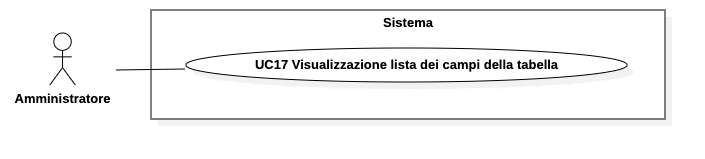
\includegraphics[scale=0.6]{UML_Use_Cases/UC17.png}
\begin{itemize}
	\item \textbf{Descrizione:} l’amministratore\textsuperscript{G} visualizza tutti i campi della tabella\textsuperscript{G} selezionata;
	\item \textbf{Attori\textsuperscript{G}:} amministratore\textsuperscript{G};
	\item \textbf{Precondizioni:} 
	\begin{itemize}
		\item L’amministratore\textsuperscript{G} ha effettuato il \textit{login\textsuperscript{G}} (\hyperref[sec:UC1]{\textbf{UC1}});
		\item L’amministratore\textsuperscript{G} si trova nella sezione di visualizzazione di una tabella\textsuperscript{G} (\hyperref[sec:UC12]{\textbf{UC12}} ;
		\item L’amministratore\textsuperscript{G} si trova nel pannello amministrativo;
	\end{itemize}
	\item \textbf{Postcondizioni:} 
	\begin{itemize}
		\item L'amministratore\textsuperscript{G} può vedere nome, tipo e sinonimi\textsuperscript{G} dei campi presenti;
	\end{itemize}
	\item \textbf{Scenario principale:} 
	\begin{itemize}
		\item Il programma visualizza la lista dei campi presenti, con la possibilità di modificarli, visualizzarli o eliminarli;
	\end{itemize}
\end{itemize}

\subsection{UC18 - Visualizzazione singolo campo\textsuperscript{G} tabella\textsuperscript{G}}
\label{sec:UC18}
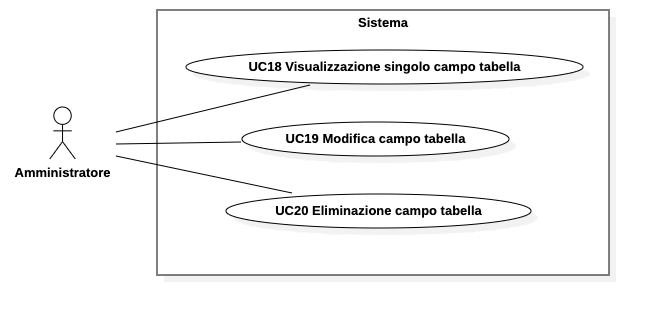
\includegraphics[scale=0.6]{UML_Use_Cases/UC18_19_20.png}
\begin{itemize}
	\item \textbf{Descrizione:} l’amministratore\textsuperscript{G} visualizza tutti i campi della tabella\textsuperscript{G} selezionata;
	\item \textbf{Attori\textsuperscript{G}:} amministratore\textsuperscript{G};
	\item \textbf{Precondizioni:} 
	\begin{itemize}
		\item L’amministratore\textsuperscript{G} ha effettuato il \textit{login\textsuperscript{G}} (\hyperref[sec:UC1]{\textbf{UC1}});
		\item L’amministratore\textsuperscript{G} si trova nella sezione di visualizzazione di una tabella\textsuperscript{G} (\hyperref[sec:UC12]{\textbf{UC12}});
		\item L’amministratore\textsuperscript{G} si trova nel pannello amministrativo;
		\item L'amministratore\textsuperscript{G} ha selezionato un campo\textsuperscript{G} di una tabella\textsuperscript{G};
	\end{itemize}
	\item \textbf{Postcondizioni:} 
	\begin{itemize}
		\item L'amministratore\textsuperscript{G} può vedere nome, tipo e sinonimi\textsuperscript{G} del campo\textsuperscript{G} selezionatoi;
	\end{itemize}
	\item \textbf{Scenario principale:} 
	\begin{itemize}
		\item Il programma visualizza la lista dei campi presenti, con la possibilità di modificarli, visualizzarli o eliminarli;
	\end{itemize}
\end{itemize}

\subsection{UC19 - Modifica campo\textsuperscript{G} tabella\textsuperscript{G}}
\label{sec:UC19}
%\includegraphics[]{diagramma_UML}
\begin{itemize}
	\item \textbf{Descrizione:} l’amministratore\textsuperscript{G} vuole modificare un campo\textsuperscript{G} alla tabella\textsuperscript{G} selezionata;
	\item \textbf{Attori\textsuperscript{G}:} amministratore\textsuperscript{G};
	\item \textbf{Precondizioni:} 
	\begin{itemize}
		\item L’amministratore\textsuperscript{G} ha effettuato il \textit{login\textsuperscript{G}} (\hyperref[sec:UC1]{\textbf{UC1}});
		\item L’amministratore\textsuperscript{G} si trova nel pannello amministrativo;
		\item L’amministratore\textsuperscript{G} si trova nella sezione di visualizzazione di una tabella\textsuperscript{G} (\hyperref[sec:UC12]{\textbf{UC12}});
		\item L’amministratore\textsuperscript{G} sta modificando i campi che compongono la tabella\textsuperscript{G};
	\end{itemize}
	\item \textbf{Postcondizioni:} 
	\begin{itemize}
		\item I campi della tabella\textsuperscript{G} vengono modificati;
	\end{itemize}
	\item \textbf{Scenario principale:} 
	\begin{itemize}
		\item L’amministratore\textsuperscript{G} inserisce il nome del campo\textsuperscript{G} \hyperref[sec:UC15.1]{\textbf{UC15.1}};
		\item L'amministratore\textsuperscript{G} seleziona il tipo del campo\textsuperscript{G} \hyperref[sec:UC15.2]{\textbf{UC15.2}};
		\item L'amministratore\textsuperscript{G} inserisce i sinonimi\textsuperscript{G} del campo\textsuperscript{G} \hyperref[sec:UC15.3]{\textbf{UC15.3}};
	\end{itemize}

		\item \textbf{Estensioni:} nel caso in cui il nome inserito sia già esistente o non sia stato selezionato il tipo o inseriti i sinonimi\textsuperscript{G}:
		\begin{itemize}
			\item (\hyperref[sec:UC16]{\textbf{UC16}}) - Errore creazione campo\textsuperscript{G}
	\end{itemize}
\end{itemize}


\subsection{UC20 - Eliminazione campo\textsuperscript{G} tabella\textsuperscript{G}}
\label{sec:UC20}
%\includegraphics[]{diagramma_UML}
\begin{itemize}
	\item \textbf{Descrizione:} l’amministratore\textsuperscript{G} elimina il campo\textsuperscript{G} selezionato;
	\item \textbf{Attori\textsuperscript{G}:} amministratore\textsuperscript{G};
	\item \textbf{Precondizioni:} 
	\begin{itemize}
		\item L’amministratore\textsuperscript{G} ha effettuato il \textit{login\textsuperscript{G}} (\hyperref[sec:UC1]{\textbf{UC1}});
		\item L’amministratore\textsuperscript{G} si trova nel pannello amministrativo;
		\item L’amministratore\textsuperscript{G} sta visualizzando la lista dei campi (\hyperref[sec:UC15]{\textbf{UC15}});
	\end{itemize}
	\item \textbf{Postcondizioni:} 
	\begin{itemize}
		\item Il campo\textsuperscript{G} selezionato viene eliminato dal sistema;
	\end{itemize}
	\item \textbf{Scenario principale:} 
	\begin{itemize}
		\item L'amministratore\textsuperscript{G} seleziona il campo\textsuperscript{G} da eliminare;
		\item Il sistema visualizza un messaggio per chiedere la conferma dell'eliminazione;
		\item Se l'amministrazione conferma l'eliminazione, il campo\textsuperscript{G} verrà rimosso dal sistema e verrà visualizzato un messaggio di avvenuta eliminazione.
	\end{itemize}
\end{itemize}

\subsection{UC21 - Caricamento Struttura \textit{Database}\textsuperscript{G} tramite file\textsuperscript{G}}
\label{sec:UC21}
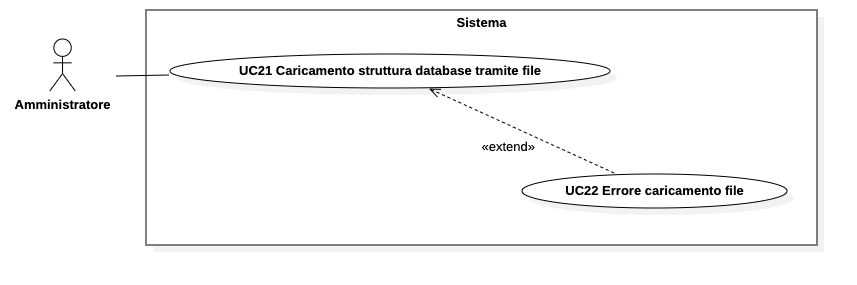
\includegraphics[scale=0.6]{UML_Use_Cases/UC21_22.png}
\begin{itemize}
	\item \textbf{Descrizione:} l’amministratore\textsuperscript{G} vuole caricare un file\textsuperscript{G} che descrive una Struttura \textit{Database}\textsuperscript{G};
	\item \textbf{Attori\textsuperscript{G}:} amministratore\textsuperscript{G};
	\item \textbf{Precondizioni:} 
	\begin{itemize}
		\item L’amministratore\textsuperscript{G} ha effettuato il \textit{login\textsuperscript{G}} (\hyperref[sec:UC1]{\textbf{UC1}});
		\item L’amministratore\textsuperscript{G} si trova nel pannello amministrativo;
	\end{itemize}
	\item \textbf{Postcondizioni:} 
	\begin{itemize}
		\item La Struttura \textit{Database}\textsuperscript{G} viene caricata correttamente nel sistema;
	\end{itemize}
	\item \textbf{Scenario principale:} 
	\begin{itemize}
		\item L'amministrazione inserisce il file\textsuperscript{G} della Struttura \textit{Database}\textsuperscript{G};
	\end{itemize}
	\item \textbf{Estensioni:} nel caso il file\textsuperscript{G} non sia corretto:
	\begin{itemize}
		\item \hyperref[sec:UC22]{\textbf{UC22}} - Errore caricamento file\textsuperscript{G}
	\end{itemize}
\end{itemize}

\subsection{UC22 - Errore caricamento file\textsuperscript{G}}
\label{sec:UC22}
\begin{itemize}
	\item \textbf{Descrizione:} L’amministratore\textsuperscript{G} visualizza un errore di caricamento del file\textsuperscript{G};
	\item \textbf{Attori\textsuperscript{G}:} amministratore\textsuperscript{G};
	\item \textbf{Precondizioni:} 
	\begin{itemize}
		\item L’amministratore\textsuperscript{G} ha effettuato il \textit{login\textsuperscript{G}} (\hyperref[sec:UC1]{\textbf{UC1}});
		\item L’amministratore\textsuperscript{G} si trova nel pannello amministrativo;
		\item L’amministratore\textsuperscript{G} sta caricando un file\textsuperscript{G} Struttura del \textit{Database} (\hyperref[sec:UC21]{\textbf{UC21}});
	\end{itemize}
	\item \textbf{Postcondizioni:} 
	\begin{itemize}
		\item La Struttura \textit{Database}\textsuperscript{G} non viene caricata e salvata, il programma visualizza un messaggio di errore;
	\end{itemize}
	\item \textbf{Scenario principale:} 
	\begin{itemize}
		\item Il sistema verifica che il formato\textsuperscript{G} del file\textsuperscript{G} sia corretto;
		\item Il sistema mostra un messaggio di errore se il formato\textsuperscript{G} non è corretto;
	\end{itemize}
\end{itemize}


\subsection{UC23 - \textit{Logout\textsuperscript{G}}}
\label{sec:UC23}
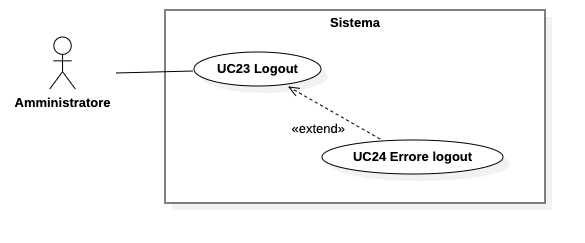
\includegraphics[scale=0.6]{UML_Use_Cases/UC23_24.png}
\begin{itemize}
	\item \textbf{Descrizione:} l'amministratore\textsuperscript{G} vuole fare il \textit{logout\textsuperscript{G}} dall'area amministrativa; 
	\item \textbf{Attori\textsuperscript{G}:} amministratore\textsuperscript{G};
	\item \textbf{Precondizioni:} 
	\begin{itemize}
		\item L’amministratore\textsuperscript{G} ha effettuato il \textit{login\textsuperscript{G}} (\hyperref[sec:UC1]{\textbf{UC1}});
	\end{itemize}
	\item \textbf{Postcondizioni:} 
	\begin{itemize}
		\item Viene visualizzata la pagina iniziale;
	\end{itemize}
	\item \textbf{Scenario principale:} 
	\begin{itemize}
		\item L’amministratore\textsuperscript{G} clicca il pulsante di \textit{logout\textsuperscript{G}};
		\item L’amministratore\textsuperscript{G} viene reindirizzato alla pagina di \textit{Login}\textsuperscript{G}.
	\end{itemize}
	\item \textbf{Estensioni:} nel caso in cui l'utente\textsuperscript{G} non fosse loggato:
	\begin{itemize}
		\item Viene visualizzato un errore - \hyperref[sec:UC24]{\textbf{UC24}}.
	\end{itemize}
\end{itemize}

\subsection{UC24 - Errore \textit{logout\textsuperscript{G}}}
\label{sec:UC24}
\begin{itemize}
	\item \textbf{Descrizione:} L’amministratore\textsuperscript{G} visualizza un errore di \textit{logout\textsuperscript{G}};
	\item \textbf{Attori\textsuperscript{G}:} amministratore\textsuperscript{G};
	\item \textbf{Precondizioni:} 
	\begin{itemize}
		\item L’amministratore\textsuperscript{G} sta tentando di fare il \textit{logout\textsuperscript{G}} (\hyperref[sec:UC21]{\textbf{UC21}});
		\item Il sistema non riescie a riconoscere un amministratore\textsuperscript{G} da scollegare;
	\end{itemize}
	\item \textbf{Postcondizioni:} 
	\begin{itemize}
		\item L'amministratore\textsuperscript{G} viene reindirizzato alla pagina di \textit{Login}\textsuperscript{G}, il programma visualizza un messaggio di errore;
	\end{itemize}
	\item \textbf{Scenario principale:} 
	\begin{itemize}
		\item Il sistema verifica la presenza di un amministratore\textsubscript{G};
		\item Il sistema mostra un messaggio di errore se non riesce ad identifare un amministratore\textsuperscript{G};
		\item L'amministratore\textsuperscript{G} viene riportato alla pagina di \textit{login}\textsuperscript{G}.
	\end{itemize}
\end{itemize}

\subsection{UC25 - Selezione Struttura \textit{Database}\textsuperscript{G} da interrogare}
\label{sec:UC25}
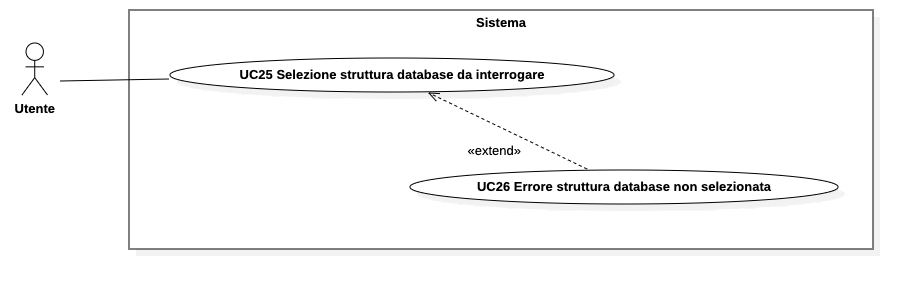
\includegraphics[scale=0.55]{UML_Use_Cases/UC25_26.png}
\begin{itemize}
	\item \textbf{Descrizione:} l’utente\textsuperscript{G} seleziona la Struttura \textit{Database}\textsuperscript{G} che vuole interrogare da una lista;
	\item \textbf{Attori\textsuperscript{G}:} utente\textsuperscript{G};
	\item \textbf{Precondizioni:}
	\begin{itemize}
		\item Sono presenti una o più Strutture \textit{Database}\textsuperscript{G} da poter selezionare;
	\end{itemize}
	\item \textbf{Postcondizioni:}
	\begin{itemize}
		\item L’utente\textsuperscript{G} ha selezionato una Struttura \textit{Database}\textsuperscript{G};
	\end{itemize}
	\item \textbf{Scenario principale:}
	\begin{itemize}
		\item L’utente\textsuperscript{G} ha il programma aperto;
		\item L’utente\textsuperscript{G} seleziona uno delle Struttura \textit{Database}\textsuperscript{G} presenti nella lista.
	\end{itemize}
	\item \textbf{Estensioni:} In caso l'utente\textsuperscript{G} non selezioni una Strttura \textit{Database};
	\begin{itemize}
		\item Errore Struttura \textit{Database}\textsuperscript{G} non selezionata (\hyperref[sec:UC26]{\textbf{UC26}});
	\end{itemize}
\end{itemize}

\subsection{UC26 - Errore Struttura \textit{Database}\textsuperscript{G} non selezionata}
\label{sec:UC26}
\begin{itemize}
	\item \textbf{Descrizione:} l’utente\textsuperscript{G} non ha selezionato una Struttura \textit{Database}\textsuperscript{G};
	\item \textbf{Attori\textsuperscript{G}:} utente\textsuperscript{G};
	\item \textbf{Precondizioni:}
	\begin{itemize}
		\item Sono presenti una o più Strutture \textit{Database}\textsuperscript{G} da poter selezionare;
	\end{itemize}
	\item \textbf{Postcondizioni:}
	\begin{itemize}
		\item L’utente\textsuperscript{G} visualizza un messaggio di errore;
	\end{itemize}
	\item \textbf{Scenario principale:}
	\begin{itemize}
		\item Il sistema non riceve una Struttura \textit{Database}\textsuperscript{G};
		\item Il sistema mostra un errore;
	\end{itemize}
\end{itemize}

\subsection{UC27 - Inserimento frase in linguaggio naturale\textsuperscript{G}}
\label{sec:UC27}
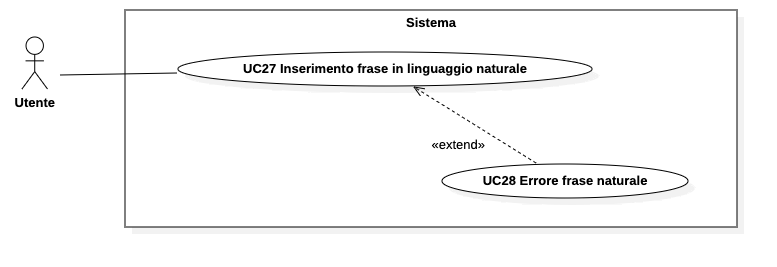
\includegraphics[scale=0.6]{UML_Use_Cases/UC27_28.png}
\begin{itemize}
	\item \textbf{Descrizione:} L’utente\textsuperscript{G} scrive una frase in linguaggio naturale\textsuperscript{G};
	\item \textbf{Attori\textsuperscript{G}:} utente\textsuperscript{G};
	\item \textbf{Precondizioni:} 
	\begin{itemize}
		\item L’utente\textsuperscript{G} ha selezionato un file\textsuperscript{G} di struttura \textit{Database}\textsuperscript{G} (\hyperref[sec:UC25]{\textbf{UC25}});
	\end{itemize}
	\item \textbf{Postcondizioni:} 
	\begin{itemize}
		\item L’utente\textsuperscript{G} riceve un \textit{prompt\textsuperscript{G}} per la creazione della \textit{query\textsuperscript{G}} richiesta (\hyperref[sec:UC29]{\textbf{UC29}});
	\end{itemize}
	\item \textbf{Scenario principale:} 
	\begin{itemize}
		\item L’utente\textsuperscript{G} ha il programma aperto;
		\item L’utente\textsuperscript{G} inserisce la frase per interrogare la Struttura \textit{Database}\textsuperscript{G};
		\item L’utente\textsuperscript{G} ottiene il \textit{prompt\textsuperscript{G}}.
	\end{itemize}
	\item \textbf{Estensioni:} nel caso in cui venga inserita una frase non inerente al \textit{database\textsuperscript{G}}, o non comprensibile:
	\begin{itemize}
		\item Viene visualizzato un errore - \hyperref[sec:UC28]{\textbf{UC28}}.
	\end{itemize}
\end{itemize}

\subsection{UC28 - Errore frase naturale}
\label{sec:UC28}
\begin{itemize}
	\item \textbf{Descrizione:} L’utente\textsuperscript{G} visualizza un errore inerente alla frase inserita;
	\item \textbf{Attori\textsuperscript{G}:} utente\textsuperscript{G};
	\item \textbf{Precondizioni:} 
	\begin{itemize}
		\item L’utente\textsuperscript{G} ha selezionato un file\textsuperscript{G} di struttura \textit{Database}\textsuperscript{G} (\hyperref[sec:UC25]{\textbf{UC25}});
		\item L'utente\textsuperscript{G} ha inserito una frase in linguaggio naturale\textsuperscript{G} (\hyperref[sec:UC27]{\textbf{UC27}});
	\end{itemize}
	\item \textbf{Postcondizioni:} 
	\begin{itemize}
		\item L’utente\textsuperscript{G} visualizza un messaggio di errore;
	\end{itemize}
	\item \textbf{Scenario principale:} 
	\begin{itemize}
		\item Il sistema verifica la frase ricevuta;
		\item Il sistema non riesce ad elaborare la frase;
		\item Il sistema visualizza un messaggio di errore.
	\end{itemize}
\end{itemize}

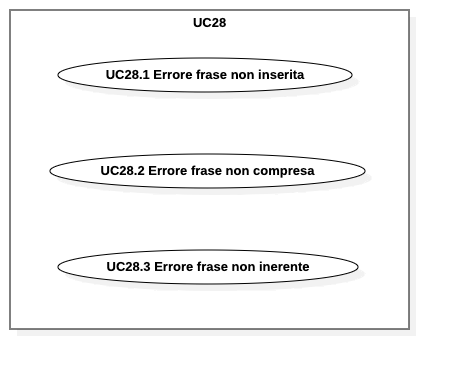
\includegraphics[scale=0.6]{UML_Use_Cases/UC28.1_28.2_28.3.png}

\subsubsection{UC28.1 - Errore frase non inserita}
\label{sec:UC28.1}
%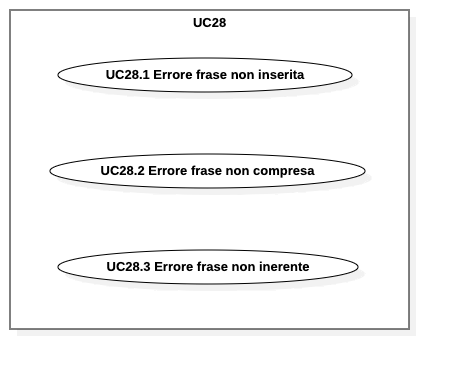
\includegraphics[scale=0.6]{UML_Use_Cases/UC28.1_28.2_28.3.png}
\begin{itemize}
	\item \textbf{Descrizione:} L’utente\textsuperscript{G} visualizza un errore relativo alla frase inserita;
	\item \textbf{Attori\textsuperscript{G}:} utente\textsuperscript{G};
	\item \textbf{Precondizioni:} 
	\begin{itemize}
		\item L’utente\textsuperscript{G} ha selezionato una Struttura \textit{Database}\textsuperscript{G} (\hyperref[sec:UC25]{\textbf{UC25}});
		\item L'utente\textsuperscript{G} ha inserito una frase in linguaggio naturale\textsuperscript{G} (\hyperref[sec:UC27]{\textbf{UC27}});
	\end{itemize}
	\item \textbf{Postcondizioni:} 
	\begin{itemize}
		\item Il programma mostra un messaggio di errore;
		\item Il \textit{prompt\textsuperscript{G}} non viene generato;
	\end{itemize}
	\item \textbf{Scenario principale:} 
	\begin{itemize}
		\item Il sistema non ha ricevuto una frase;
		\item Il sistema visualizza un messaggio di errore.
	\end{itemize}
\end{itemize}


\subsubsection{UC28.2 - Errore frase non compresa}
\label{sec:UC28.2}
\begin{itemize}
	\item \textbf{Descrizione:} L’utente\textsuperscript{G} inserisce una frase in linguaggio naturale\textsuperscript{G} non comprensibile dal sistema;
	\item \textbf{Attori\textsuperscript{G}:} utente\textsuperscript{G};
	\item \textbf{Precondizioni:} 
	\begin{itemize}
			\item L’utente\textsuperscript{G} ha selezionato una Struttura \textit{Database}\textsuperscript{G} (\hyperref[sec:UC25]{\textbf{UC25}});
		\item L'utente\textsuperscript{G} ha inserito una frase in linguaggio naturale\textsuperscript{G} (\hyperref[sec:UC27]{\textbf{UC27}});
	\end{itemize}
	\item \textbf{Postcondizioni:} 
	\begin{itemize}
		\item Il programma mostra un messaggio di errore;
		\item Il \textit{prompt\textsuperscript{G}} non viene generato;
	\end{itemize}
	\item \textbf{Scenario principale:} 
	\begin{itemize}
		\item Il sistema verifica la frase ricevuta;
		\item Il sistema non comprende la frase;
		\item Il sistema visualizza un messaggio di errore.
	\end{itemize}
\end{itemize}


\subsubsection{UC28.3 - Errore frase non inerente}
\label{sec:UC28.3}
%\includegraphics[]{diagramma_UML}
\begin{itemize}
	\item \textbf{Descrizione:} l’utente\textsuperscript{G} inserisce una frase in linguaggio naturale\textsuperscript{G} non interpretabile dal sistema come inerente al \textit{database\textsuperscript{G}};
	\item \textbf{Attori\textsuperscript{G}:} utente\textsuperscript{G};
	\item \textbf{Precondizioni:} 
	\begin{itemize}
			\item L’utente\textsuperscript{G} ha selezionato una Struttura \textit{Database}\textsuperscript{G} (\hyperref[sec:UC25]{\textbf{UC25}});
		\item L’utente\textsuperscript{G} ha scritto una frase in linguaggio naturale\textsuperscript{G} nella casella di testo apposita e ne ha confermato l’inserimento (\hyperref[sec:UC27]{\textbf{UC24}});
	\end{itemize}
	\item \textbf{Postcondizioni:} 
	\begin{itemize}
		\item Il programma mostra un messaggio di errore;
		\item Il \textit{prompt\textsuperscript{G}} non viene generato;
	\end{itemize}
	\item \textbf{Scenario principale:} 
	\begin{itemize}
		\item Il sistema verifica la frase ricevuta;
		\item Il sistema non trova componenti inerenti alla Struttura \textit{Database}\textsuperscript{G} nella frase;
		\item Il sistema visualizza un messaggio di errore.
	\end{itemize}
\end{itemize}

\subsection{UC29 - Visualizzazione \textit{prompt\textsuperscript{G}} generato}
\label{sec:UC29}
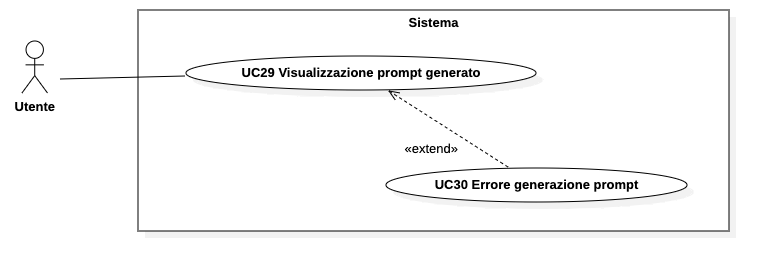
\includegraphics[scale=0.6]{UML_Use_Cases/UC29_30.png}
\begin{itemize}
	\item \textbf{Descrizione:} L’utente\textsuperscript{G} riceve il \textit{prompt\textsuperscript{G}} per la generazione della \textit{query\textsuperscript{G}};
	\item \textbf{Attori\textsuperscript{G}:} utente\textsuperscript{G};
	\item \textbf{Precondizioni:} 
	\begin{itemize}
		\item L’utente\textsuperscript{G} ha selezionato una Struttura \textit{Database}\textsuperscript{G} (\hyperref[sec:UC25]{\textbf{UC25}});
		\item L’utente\textsuperscript{G} ha scritto una frase in linguaggio naturale\textsuperscript{G} (\hyperref[sec:UC27]{\textbf{UC24}});
	\end{itemize}
	\item \textbf{Postcondizioni:} 
	\begin{itemize}
		\item Il programma visualizza il \textit{prompt\textsuperscript{G}} per la creazione della \textit{query\textsuperscript{G}} richiesta;
	\end{itemize}
	\item \textbf{Scenario principale:} 
	\begin{itemize}
		\item L’utente\textsuperscript{G} ha il programma aperto;
		\item L’utente\textsuperscript{G} ha selezionato una Struttura \textit{Database}\textsuperscript{G} (\hyperref[sec:UC25]{\textbf{UC25}})
		\item L'utente\textsuperscript{G} ha inserito la frase in linguaggio naturale\textsuperscript{G} (\hyperref[sec:UC27]{\textbf{UC27}});
		\item L’utente\textsuperscript{G} richiede il \textit{prompt\textsuperscript{G}};
		\item Il programma visualizza il \textit{prompt\textsuperscript{G}} elaborato.
	\end{itemize}
	\item \textbf{Estensioni:} nel caso in cui non sia possibile generare il \textit{prompt\textsuperscript{G}}:
	\begin{itemize}
		\item Viene visualizzato un errore - \hyperref[sec:UC30]{\textbf{UC30}}.
	\end{itemize}
\end{itemize}

\subsection{UC30 - Errore generazione \textit{prompt\textsuperscript{G}}}
\label{sec:UC30}
\begin{itemize}
	\item \textbf{Descrizione:} L’utente\textsuperscript{G} visualizza un errore inerente alla generazione del \textit{prompt\textsuperscript{G}};
	\item \textbf{Attori\textsuperscript{G}:} utente\textsuperscript{G};
	\item \textbf{Precondizioni:} 
	\begin{itemize}
		\item L’utente\textsuperscript{G} ha selezionato un file\textsuperscript{G} di struttura \textit{Database}\textsuperscript{G} (\hyperref[sec:UC25]{\textbf{UC25}});
		\item L’utente\textsuperscript{G} ha scritto una frase in linguaggio naturale\textsuperscript{G} (\hyperref[sec:UC27]{\textbf{UC27}});
		\item L’utente\textsuperscript{G} richiede il \textit{prompt\textsuperscript{G}};
	\end{itemize}
	\item \textbf{Postcondizioni:} 
	\begin{itemize}
		\item L’utente\textsuperscript{G} visualizza un messaggio di errore;
	\end{itemize}
	\item \textbf{Scenario principale:} 
	\begin{itemize}
		\item Il sistema verifica il \textit{prompt\textsuperscript{G}} e ritorna l'errore adeguato;
	\end{itemize}
\end{itemize}

\subsubsection{UC30.1 - Errore comunicazione con \textit{LLM\textsuperscript{G}}}
\label{sec:UC30.1}
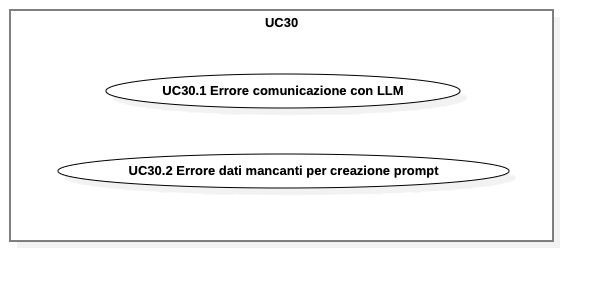
\includegraphics[scale=0.6]{UML_Use_Cases/UC30.1_30.2.png}
\begin{itemize}
	\item \textbf{Descrizione:} L’utente\textsuperscript{G} visualizza un errore inerente alla comunicazione con il modello\textsuperscript{G} \textit{LLM\textsuperscript{G}};
	\item \textbf{Attori\textsuperscript{G}:} utente\textsuperscript{G};
	\item \textbf{Precondizioni:} 
	\begin{itemize}
		\item L’utente\textsuperscript{G} ha selezionato un file\textsuperscript{G} di struttura \textit{Database}\textsuperscript{G} (\hyperref[sec:UC25]{\textbf{UC25}});
		\item L’utente\textsuperscript{G} ha scritto una frase in linguaggio naturale\textsuperscript{G} (\hyperref[sec:UC27]{\textbf{UC27}});
		\item L’utente\textsuperscript{G} richiede il \textit{prompt\textsuperscript{G}};
	\end{itemize}
	\item \textbf{Postcondizioni:} 
	\begin{itemize}
		\item L’utente\textsuperscript{G} visualizza un messaggio di errore;
	\end{itemize}
	\item \textbf{Scenario principale:} 
	\begin{itemize}
		\item Il sistema riceve il \textit{prompt\textsuperscript{G}};
		\item Il sistema non riesce a comunicare con il modello\textsuperscript{G} \textit{LLM\textsuperscript{G}};
		\item Il sistema mostra un errore;
	\end{itemize}
\end{itemize}

\subsubsection{UC30.2 - Errore dati mancanti per creazione \textit{prompt\textsuperscript{G}}}
\label{sec:UC30.2}
\begin{itemize}
	\item \textbf{Descrizione:} L’utente\textsuperscript{G} visualizza un errore inerente alla frase in linguaggio naturale\textsuperscript{G};
	\item \textbf{Attori\textsuperscript{G}:} utente\textsuperscript{G};
	\item \textbf{Precondizioni:} 
	\begin{itemize}
		\item L’utente\textsuperscript{G} ha selezionato un file\textsuperscript{G} di struttura \textit{Database}\textsuperscript{G} (\hyperref[sec:UC25]{\textbf{UC25}});
		\item L’utente\textsuperscript{G} ha scritto una frase in linguaggio naturale\textsuperscript{G} (\hyperref[sec:UC27]{\textbf{UC27}});
		\item L’utente\textsuperscript{G} richiede il \textit{prompt\textsuperscript{G}};
	\end{itemize}
	\item \textbf{Postcondizioni:} 
	\begin{itemize}
		\item L’utente\textsuperscript{G} visualizza un messaggio di errore;
	\end{itemize}
	\item \textbf{Scenario principale:} 
	\begin{itemize}
		\item Il sistema riceve il \textit{prompt\textsuperscript{G}};
		\item Il sistema non trova tutti i dati necessari per la generazione del \textit{prompt\textsuperscript{G}} ;
		\item Il sistema mostra un errore;
	\end{itemize}
\end{itemize}

\subsection{UC31 - Richiesta generazione \textit{query SQL}\textsuperscript{G}}
\label{sec:UC31}
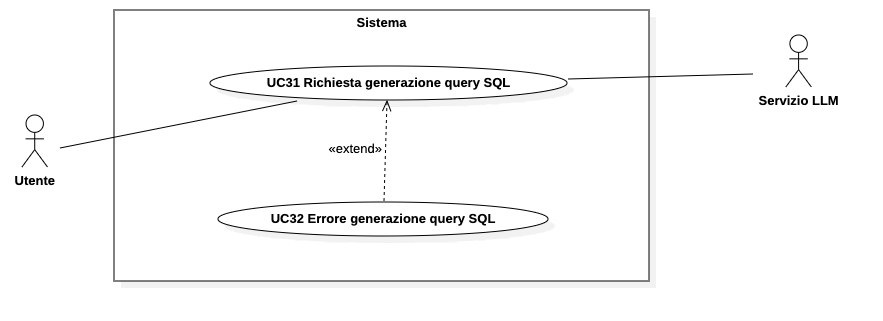
\includegraphics[scale=0.55]{UML_Use_Cases/UC31_32.png}
\begin{itemize}
    \item \textbf{Descrizione:} L'utente\textsuperscript{G} richiede la generazione della \textit{query SQL\textsuperscript{G}};
    \item \textbf{Attori\textsuperscript{G}:} utente\textsuperscript{G}, Servizio \textit{LLM}\textsuperscript{G};
    \item \textbf{Precondizioni:} 
    \begin{itemize}
    	\item L'utente\textsuperscript{G} ha visualizzato il \textit{prompt\textsuperscript{G}} (\hyperref[sec:UC29]{\textbf{UC29}});
    \end{itemize}
    \item \textbf{Postcondizioni:} 
    \begin{itemize}
    	\item L'utente\textsuperscript{G} visualizza la \textit{query SQL\textsuperscript{G}} richiesta (\hyperref[sec:UC33]{\textbf{UC33}});
    \end{itemize}
    \item \textbf{Scenario principale:}
    \begin{itemize}
    	\item L'utente\textsuperscript{G} richiede la generazione della \textit{query SQL\textsuperscript{G}} a partire dal \textit{prompt\textsuperscript{G}} ricevuto;
    	\item Il sistema verifica il \textit{prompt\textsuperscript{G}} ricevuto;
    	\item Il sistema invia il \textit{prompt\textsuperscript{G}} al servizio \textit{LLM\textsuperscript{G}} esterno;
    \end{itemize}
    \item \textbf{Estensioni:} In caso non sia possibile generare la \textit{query SQL\textsuperscript{G}}:
    \begin{itemize}
    	\item Errore generazione \textit{query SQL\textsuperscript{G}} (\hyperref[sec:UC32]{\textbf{UC32}});
    \end{itemize}
\end{itemize}

\subsection{UC32 - Errore generazione \textit{query SQL\textsuperscript{G}}}
\label{sec:UC32}
%   \includegraphics[]{diagramma_UML}
\begin{itemize}
	\item \textbf{Descrizione:} L'utente\textsuperscript{G} visualizza un messaggio di errore inerente alla generazione della \textit{query SQL\textsuperscript{G}};
	\item \textbf{Attori\textsuperscript{G}:} utente\textsuperscript{G}, Servizio \textit{LLM}\textsuperscript{G};
	\item \textbf{Precondizioni:} 
	\begin{itemize}
		\item L'utente\textsuperscript{G} ha visualizzato il \textit{prompt\textsuperscript{G}} (\hyperref[sec:UC29]{\textbf{UC29}});
		\item L'utente\textsuperscript{G} richiede la generazione della \textit{query\textsuperscript{G} SQL\textsuperscript{G}} (\hyperref[sec:UC31]{\textbf{UC31}});
	\end{itemize}
	\item \textbf{Postcondizioni:} 
	\begin{itemize}
		\item L'utente\textsuperscript{G} visualizza un messaggio di errore;
	\end{itemize}
	\item \textbf{Scenario principale:}
	\begin{itemize}
		\item L'utente\textsuperscript{G} richiede la generazione della \textit{query SQL\textsuperscript{G}} a partire dal \textit{prompt\textsuperscript{G}} ricevuto;
		\item Il sistema verifica il \textit{prompt\textsuperscript{G}} ricevuto;
		\item Il sistema invia il \textit{prompt\textsuperscript{G}} al servizio \textit{LLM\textsuperscript{G}} esterno;
		\item Il sistema mostra un messaggio di errore;
	\end{itemize}
\end{itemize}

\subsubsection{UC32.1 - Errore comunicazione con API\textsuperscript{G}}
\label{sec:UC32.1}
\includegraphics[scale=0.6]{UML_Use_Cases/UC32.1_32.2.png}
\begin{itemize}
	\item \textbf{Descrizione:} L'utente\textsuperscript{G} visualizza un messaggio di errore inerente alla comunicazione con il servizio di API\textsuperscript{G} esterno;
	\item \textbf{Attori\textsuperscript{G}:} utente\textsuperscript{G}, Servizio \textit{LLM}\textsuperscript{G};
	\item \textbf{Precondizioni:} 
	\begin{itemize}
		\item L'utente\textsuperscript{G} ha visualizzato il \textit{prompt\textsuperscript{G}} (\hyperref[sec:UC29]{\textbf{UC29}});
		\item L'utente\textsuperscript{G} richiede la generazione della \textit{query\textsuperscript{G} SQL\textsuperscript{G}} (\hyperref[sec:UC31]{\textbf{UC31}});
	\end{itemize}
	\item \textbf{Postcondizioni:} 
	\begin{itemize}
		\item L'utente\textsuperscript{G} un messaggio di errore;
	\end{itemize}
	\item \textbf{Scenario principale:}
	\begin{itemize}
		\item L'utente\textsuperscript{G} richiede la generazione della \textit{query SQL\textsuperscript{G}} a partire dal \textit{prompt\textsuperscript{G}} ricevuto;
		\item Il sistema verifica il \textit{prompt\textsuperscript{G}} ricevuto;
		\item Il sistema invia il \textit{prompt\textsuperscript{G}} al servizio \textit{LLM\textsuperscript{G}} esterno;
		\item Il sistema non riesce a comunicare con il servizio \textit{LLM\textsuperscript{G}} esterno;
		\item Il sistema mostra un messaggio di errore;
	\end{itemize}
\end{itemize}

\subsubsection{UC32.2 - Errore formattazione \textit{prompt\textsuperscript{G}}}
\label{sec:UC32.2}
\begin{itemize}
	\item \textbf{Descrizione:} L'utente\textsuperscript{G} visualizza un messaggio di errore inerente alla formattazione del \textit{prompt\textsuperscript{G}} creato;
	\item \textbf{Attori\textsuperscript{G}:} utente\textsuperscript{G}, Servizio \textit{LLM}\textsuperscript{G};
	\item \textbf{Precondizioni:} 
	\begin{itemize}
		\item L'utente\textsuperscript{G} ha visualizzato il \textit{prompt\textsuperscript{G}} (\hyperref[sec:UC29]{\textbf{UC29}});
		\item L'utente\textsuperscript{G} richiede la generazione della \textit{query SQL\textsuperscript{G}} (\hyperref[sec:UC31]{\textbf{UC31}});
	\end{itemize}
	\item \textbf{Postcondizioni:} 
	\begin{itemize}
		\item L'utente\textsuperscript{G} visualizza un messaggio di errore;
	\end{itemize}
	\item \textbf{Scenario principale:}
	\begin{itemize}
		\item L'utente\textsuperscript{G} richiede la generazione della \textit{query SQL\textsuperscript{G}} a partire dal \textit{prompt\textsuperscript{G}} ricevuto;
		\item Il sistema verifica il \textit{prompt\textsuperscript{G}} ricevuto;
		\item Il sistema invia il \textit{prompt\textsuperscript{G}} al servizio \textit{LLM\textsuperscript{G}} esterno;
		\item Il sistema riceve un errore dal servizio \textit{LLM\textsuperscript{G}} esterno;
		\item Il sistema mostra un messaggio di errore;
	\end{itemize}
\end{itemize}

\subsection{UC33 - Visualizzazione \textit{query SQL\textsuperscript{G}}}
\label{sec:UC33}
\begin{itemize}
	\item \textbf{Descrizione:} L’utente\textsuperscript{G} visualizza la \textit{query SQL\textsuperscript{G}} ricevuta dal servizio \textit{LLM\textsuperscript{G}} esterno;
	\item \textbf{Attori\textsuperscript{G}:} utente\textsuperscript{G}, Servizio \textit{LLM}\textsuperscript{G};
	\item \textbf{Precondizioni:} 
	\begin{itemize}
		\item L’utente\textsuperscript{G} ha selezionato una \textsuperscript{G} di struttura \textit{Database}\textsuperscript{G} (\hyperref[sec:UC25]{\textbf{UC25}});
		\item L’utente\textsuperscript{G} ha inserito una frase in linguaggio naturale\textsuperscript{G} (\hyperref[sec:UC27]{\textbf{UC27}});
		\item Il programma visualizza il \textit{prompt\textsuperscript{G}} elaborato (\hyperref[sec:UC29]{\textbf{UC29}});
		\item L’utente\textsuperscript{G} richiesto la generazione della \textit{query SQL\textsuperscript{G}} (\hyperref[sec:UC31]{\textbf{UC31}});
	\end{itemize}
	\item \textbf{Postcondizioni:} 
	\begin{itemize}
		\item Il programma visualizza la \textit{query SQL\textsuperscript{G}} richiesta;
	\end{itemize}
	\item \textbf{Scenario principale:} 
	\begin{itemize}
		\item L'utente\textsuperscript{G} richiede la generazione della \textit{query SQL\textsuperscript{G}} (\hyperref[sec:UC31]{\textbf{UC31}});
		\item L'utente\textsuperscript{G} visualizza la \textit{query SQL\textsuperscript{G}} richiesta;
	\end{itemize}
\end{itemize}
